\documentclass[UTF8,a4paper,12pt]{ctexart}
\usepackage{geometry}
\usepackage{array}
\usepackage{booktabs}
\usepackage{longtable}
\usepackage{tabularx}
\usepackage{xcolor}
\usepackage{listings}
\usepackage{hyperref}
\usepackage{fancyhdr}
\usepackage{enumitem}
\usepackage{titlesec}
\usepackage{caption}
\usepackage{graphicx}

\geometry{left=2.5cm,right=2.5cm,top=2.5cm,bottom=2.5cm}
\pagestyle{fancy}
\setlength{\headheight}{15pt}
\fancyhf{}
\lhead{《单片机原理及应用》PBL项目合作学习作业}
\rhead{C8051F310科创集市项目}
\cfoot{\thepage}
\hypersetup{colorlinks=true,linkcolor=blue,urlcolor=blue}
\setlist{itemsep=0.2em,topsep=0.3em}
\titleformat{\section}{\Large\bfseries}{\chinese{section}、}{0em}{}
\titleformat{\subsection}{\large\bfseries}{\arabic{subsection}.}{0.5em}{}
\renewcommand\arraystretch{1.35}

\lstdefinestyle{asmstyle}{
  basicstyle=\ttfamily\scriptsize,
  keywordstyle=\color{blue!60!black},
  commentstyle=\color{green!40!black},
  frame=single,
  breaklines=true,
  columns=fullflexible,
  keepspaces=true,
  showstringspaces=false,
  numbers=left,
  numberstyle=\tiny\color{gray},
  tabsize=4
}

\begin{document}

\begin{center}
{\zihao{2}\bfseries 《单片机原理及应用》PBL项目合作学习作业}\par
\vspace{0.4em}
{\zihao{3}\bfseries 基于C8051F310单片机的科创集市项目设计}\par
\vspace{1.2em}
\begin{tabular}{rl}
日期： & 2026-06-19 \\
专业班级： & 光电信息科学与工程202409 \\
小组成员： & 陈恪瑾（组长）、熊辰志、黄伟峰、安礼辰 \\
小组队名： & 闪电神经元队 \\
作品名称： & 基于C8051F310的反应力与节奏挑战训练仪 \\
\end{tabular}
\end{center}

\vspace{1em}
\noindent\textbf{作品一句话描述：}利用C8051F310开发板的数码管、矩阵键盘、LED流水灯、蜂鸣器、外部触发键和UART串口，设计一台可现场互动的反应力与节奏挑战小游戏原型机，完成成绩显示、声光反馈、模式切换、键盘难度设置和串口状态输出。

\section{思考题解答}

\subsection{C8051F310单片机有哪些新特性？}
C8051F310是Silicon Labs推出的混合信号SoC型单片机，内部采用高速流水线结构的CIP-51内核，与MCS-51指令集完全兼容，但指令执行效率显著高于传统8051。它集成了片内Flash、片内RAM、多个定时器、增强型UART、SPI、SMBus/I2C、10位ADC、模拟比较器、片内温度传感器、片内高精度振荡器、上电复位、VDD监视器、看门狗定时器和片内调试接口。与传统8051相比，它不仅保留了8051的软件生态和汇编开发方式，还把数据采集、控制、通信、调试和复位监控等功能集中在一颗芯片内，适合制作小型测控系统和教学综合实验项目。

从开发角度看，C8051F310的重要新特性包括：第一，CIP-51内核最高可达约25MIPS，适合更高实时性任务；第二，端口I/O具有交叉开关配置机制，可把UART、外部中断等数字外设灵活映射到引脚；第三，每个端口可配置为模拟输入、数字输入、开漏输出或推挽输出；第四，片上ADC可以直接采集模拟电压；第五，片内调试接口支持在线下载和调试，降低了实验开发难度。

\subsection{C8051F310的指令执行时间和传统8051单片机的区别是什么？}
传统8051通常以机器周期为基本时序单位，一个机器周期一般等于12个振荡周期，多数指令需要1个或2个机器周期，即12个或24个时钟周期。C8051F310的CIP-51内核采用流水线结构，指令时序直接以系统时钟周期计算。资料中指出，CIP-51约70\%的指令执行时间为1个或2个系统时钟周期，只有少数指令执行时间超过4个系统时钟周期。

因此，在相同或相近的系统时钟频率下，C8051F310的指令执行速度明显高于传统8051。对本项目而言，这种高速特性有利于实现1ms级定时、数码管动态刷新、键盘快速扫描、LED节奏控制、软件PWM调光和串口发送等并行感较强的任务。

\subsection{C8051F310单片机定时器的时钟有哪些选择？}
C8051F310内部具有多个定时器/计数器。T0和T1兼容传统8051定时器结构，可以工作在多种模式，并可选择系统时钟、由CKCON分频得到的时钟或外部计数输入。T2和T3是增强型自动重装载定时器，可作为16位自动重装载定时器，也可拆分为两个8位自动重装载定时器。T2/T3的时钟一般可以选择SYSCLK、SYSCLK/12或外部振荡源/8。

本项目使用Timer0作为周期性中断时间基准。开发板片内主频为24.5MHz，程序将Timer0配置为16位定时器，并选择SYSCLK/12作为Timer0时钟。此时Timer0计数频率约为2.041666MHz，1ms约需要2042个计数，因此重装值设置为0xF806，形成近似1ms的系统节拍。该节拍用于反应时间计数、键盘消抖、数码管刷新和游戏状态推进。

\subsection{Configuration Wizard提供图形化配置方法，请按照实验3需求配置IO口。}
结合实验3键盘数码管需求和本项目功能，IO口配置如下：

\begin{longtable}{>{\centering\arraybackslash}p{3cm}p{4cm}p{7cm}}
\toprule
引脚/端口 & 配置方式 & 用途说明 \\
\midrule
P1.0--P1.7 & 推挽输出 & 数码管段选，输出a、b、c、d、e、f、g、dp段码 \\
P0.6、P0.7 & 推挽输出 & 数码管位选A、B，选择4位数码管中的当前一位 \\
P2.0--P2.3 & 数字输出 & 4x4矩阵键盘行扫描输出KO.0--KO.3 \\
P2.4--P2.7 & 数字输入 & 4x4矩阵键盘列输入KI.0--KI.3 \\
P3.1 & 推挽输出 & 蜂鸣器控制，高电平有效 \\
P3.2 & 普通数字输入/保留 & 本项目当前版本未使用，可作为后续模拟量扩展接口 \\
P3.3 & 推挽输出 & LED流水灯74HCT164串行数据DAT\_IN \\
P3.4 & 推挽输出 & LED流水灯74HCT164移位时钟CLK \\
P0.1 & 数字输入/外部中断 & 独立触发键KINT，低电平有效，用于开始/下一轮 \\
P0.4 & UART0 TXD & 串口发送开始、成绩和失败等状态信息到电脑 \\
P0.5 & UART0 RXD & UART接收脚保留，当前程序未使用接收功能 \\
\bottomrule
\end{longtable}

Configuration Wizard中需要注意：P1设置为推挽输出以保证数码管段选驱动能力；P2低四位作为矩阵键盘行扫描输出，高四位作为列输入并依靠弱上拉保持空闲高电平；P3.1、P3.3、P3.4设置为推挽输出，用于蜂鸣器和74HCT164流水灯驱动。启用UART0后，P0.4和P0.5作为TXD/RXD使用；启用交叉开关后，普通端口输出驱动才会正常工作。

\subsection{C8051F310单片机称为SoC的原因是什么？}
SoC即System on Chip，含义是把一个完整系统所需的核心功能集成到同一芯片中。C8051F310不仅有CPU内核，还集成了程序存储器Flash、数据存储器RAM、特殊功能寄存器、通用I/O、定时器、UART/SPI/SMBus通信接口、ADC、比较器、温度传感器、振荡器、复位电路、电源监测、看门狗和在线调试接口。它能够独立完成采集、运算、控制、显示、通信等任务。

本项目正体现了SoC的价值：反应力游戏需要定时、键盘输入、数码管显示、LED驱动、蜂鸣器输出和UART通信，这些功能都可以围绕C8051F310一颗芯片完成，不需要再外接复杂的控制器。

\subsection{人工智能时代单片机可能的发展趋势。}
人工智能时代的单片机将从传统的简单控制器，逐步发展为边缘智能节点。其趋势包括：第一，片上算力继续提升，部分MCU会集成轻量化AI加速单元，用于关键词识别、异常检测、姿态识别和传感数据分类；第二，模拟前端和传感接口更丰富，便于直接连接环境、人体和工业传感器；第三，低功耗能力更强，适合长时间运行的可穿戴设备、智能家居和物联网节点；第四，通信能力增强，更多MCU会集成蓝牙、Wi-Fi、LoRa或更安全的有线通信；第五，开发工具更加智能化，AI可以辅助生成配置代码、检查寄存器设置、分析波形和定位程序错误。

对于教学而言，未来单片机学习不仅要掌握寄存器、定时器和I/O控制，也要理解如何把单片机作为智能系统中的边缘执行端和数据采集端。本项目虽然不直接运行AI模型，但通过反应数据采集、键盘难度设置和串口状态输出，体现了边缘设备采集数据、做出反馈并与上位机协同的基本思路。

\section{作品设计方案}

\subsection{项目背景与意义}
校园科创集市强调作品的可演示性、互动性和创造性。传统单片机实验通常围绕流水灯、数码管显示、键盘输入等单项功能展开，观众不容易直观看出系统设计的完整性。本项目把这些基础实验资源组合成一个可参与、可竞争、可展示成绩的互动挑战装置：反应力与节奏挑战训练仪。

在实际应用价值方面，反应力训练可用于课间娱乐、注意力训练和简单运动反应测试；节奏挑战可训练用户的节拍感和手眼协调能力。在教学意义方面，本作品覆盖了C8051F310开发板的主要数字I/O资源，能够综合考察小组成员对I/O配置、定时器中断、键盘扫描、动态显示、蜂鸣器控制、LED串行驱动和UART通信的理解。相比单一实验，本项目更接近一个完整嵌入式原型机，适合用于科创集市现场动态演示。

\subsection{功能需求分析}
\textbf{核心功能如下：}
\begin{enumerate}
  \item 反应力测试：系统随机等待后显示目标键，玩家按下正确键后，数码管显示反应时间，单位为ms。
  \item 节奏挑战：LED流水灯按节奏移动，玩家需要在随机指定的目标灯亮起时按K0得分，达到20分通关。
  \item 模式切换：K15在反应力测试和节奏挑战之间切换，KINT用于开始游戏或进入下一轮。
  \item 难度设置：在节奏模式下，K10、K11、K12分别设置低、中、高三档难度，三档均要求在目标灯单点命中，区别为流水灯移动速度不同。
  \item 数码管显示：反应模式显示目标数字和反应时间；节奏模式显示\texttt{LxSS}，其中x为本局目标灯编号，SS为当前分数。
  \item 声光反馈：蜂鸣器提示开始、成功、失败和超时；LED显示等待动画、节奏进度和成功动画。
  \item UART状态输出：通过P0.4/P0.5串口向电脑发送START、SCORE和FAIL等状态信息，便于调试和现场观察。
\end{enumerate}

\textbf{安全与交互约束如下：}
\begin{enumerate}
  \item 误按惩罚：目标出现前抢按或按错键时，本轮判定失败。
  \item 按键消抖：矩阵键盘和KINT均进行软件消抖，避免一次机械按键被重复识别。
  \item 结果保持：成功后保持反应时间或分数显示，失败后保持\texttt{FErr}提示，直到用户再次按KINT开始下一轮。
  \item LED调光：流水灯采用软件PWM降低亮度，避免现场演示时LED过亮影响观察。
\end{enumerate}

\subsection{系统总体设计}

\begin{center}
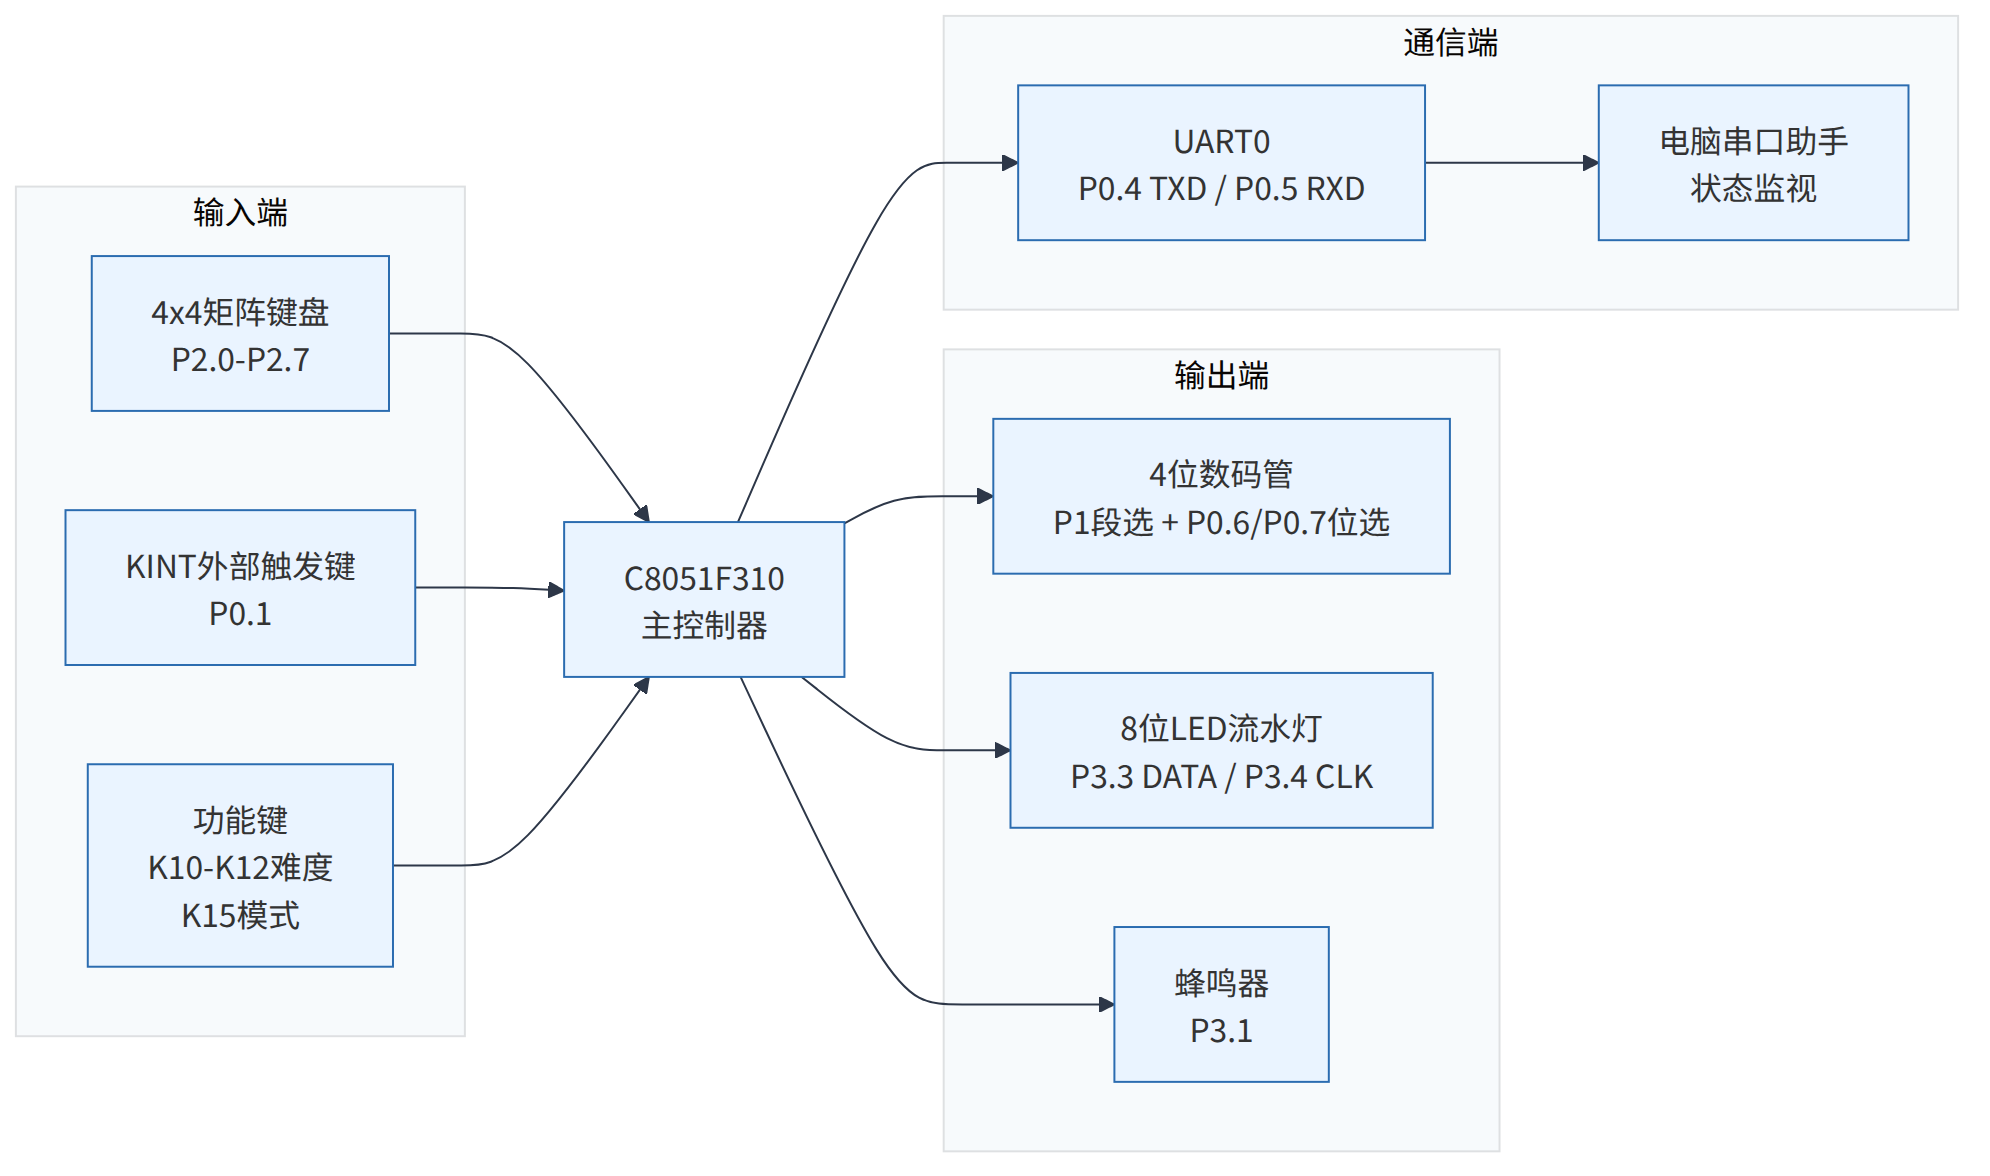
\includegraphics[width=\textwidth,height=0.86\textheight,keepaspectratio]{figures/system_architecture.png}
\captionof{figure}{系统总体硬件框图}
\end{center}

系统采用“定时器中断+主循环状态机”的软件结构。Timer0在24.5MHz片内时钟下通过0xF806重装值提供显示刷新、蜂鸣器和LED软件PWM服务；Timer2作为1ms自动重装载定时器，负责随机等待倒计时、反应时间计数和节奏模式的流水灯节拍。主循环根据状态变量执行待机、模式选择、难度设置、随机等待、显示目标、等待按键、成功反馈、失败反馈和串口状态输出等流程。

程序采用模块化工程结构。\texttt{reaction\_game.asm}作为顶层入口，统一包含公共定义和各个功能模块；\texttt{reaction\_game.inc}集中保存常量和内部RAM地址；其余模块分别承担向量表、初始化、主循环、游戏逻辑、中断、显示、键盘、随机数、LED、串口和查找表等职责。模块划分如表\ref{tab:code-modules}所示。

\begin{longtable}{>{\centering\arraybackslash\small}p{4.4cm}p{8.6cm}}
\caption{核心代码模块划分}\label{tab:code-modules}\\
\toprule
文件 & 主要职责 \\
\midrule
\texttt{Inc/reaction\_game.inc} & 定义Timer重装值、状态常量、模式常量、按键常量、数码管索引和内部RAM固定地址。 \\
\texttt{Src/reaction\_game.asm} & 顶层汇编入口，通过\texttt{\$include}组合公共定义和各个功能模块，并在文件末尾统一结束。 \\
\texttt{Src/vectors.asm} & 放置复位向量、INT0向量、Timer0向量和Timer2向量。 \\
\texttt{Src/init.asm} & 完成看门狗关闭、振荡器、端口、Timer0、Timer2、UART0初始化，并进入主循环。 \\
\texttt{Src/main.asm} & 扫描KINT和矩阵键盘，根据当前状态分发到对应状态处理函数。 \\
\texttt{Src/game\_logic.asm} & 实现反应模式、节奏模式、模式切换、难度设置、成功失败判定等核心状态机。 \\
\texttt{Src/isr.asm} & Timer0负责显示刷新、蜂鸣器和LED PWM；Timer2负责1ms计时、等待倒计时和节奏步进。 \\
\texttt{Src/display.asm} & 实现数码管动态扫描、段码查表、反应时间显示和节奏分数显示。 \\
\texttt{Src/keypad.asm} & 实现4x4矩阵键盘扫描、软件消抖、按键释放等待和KINT扫描。 \\
\texttt{Src/led\_bar.asm} & 通过P3.3/P3.4驱动74HCT164，完成LED流水灯输出和软件PWM调光。 \\
\texttt{Src/uart.asm} & 实现UART字符发送、字符串发送、成绩发送和失败状态发送。 \\
\texttt{Src/tables.asm} & 保存数码管段码表、节奏目标LED表和UART字符串。 \\
\bottomrule
\end{longtable}

\begin{center}
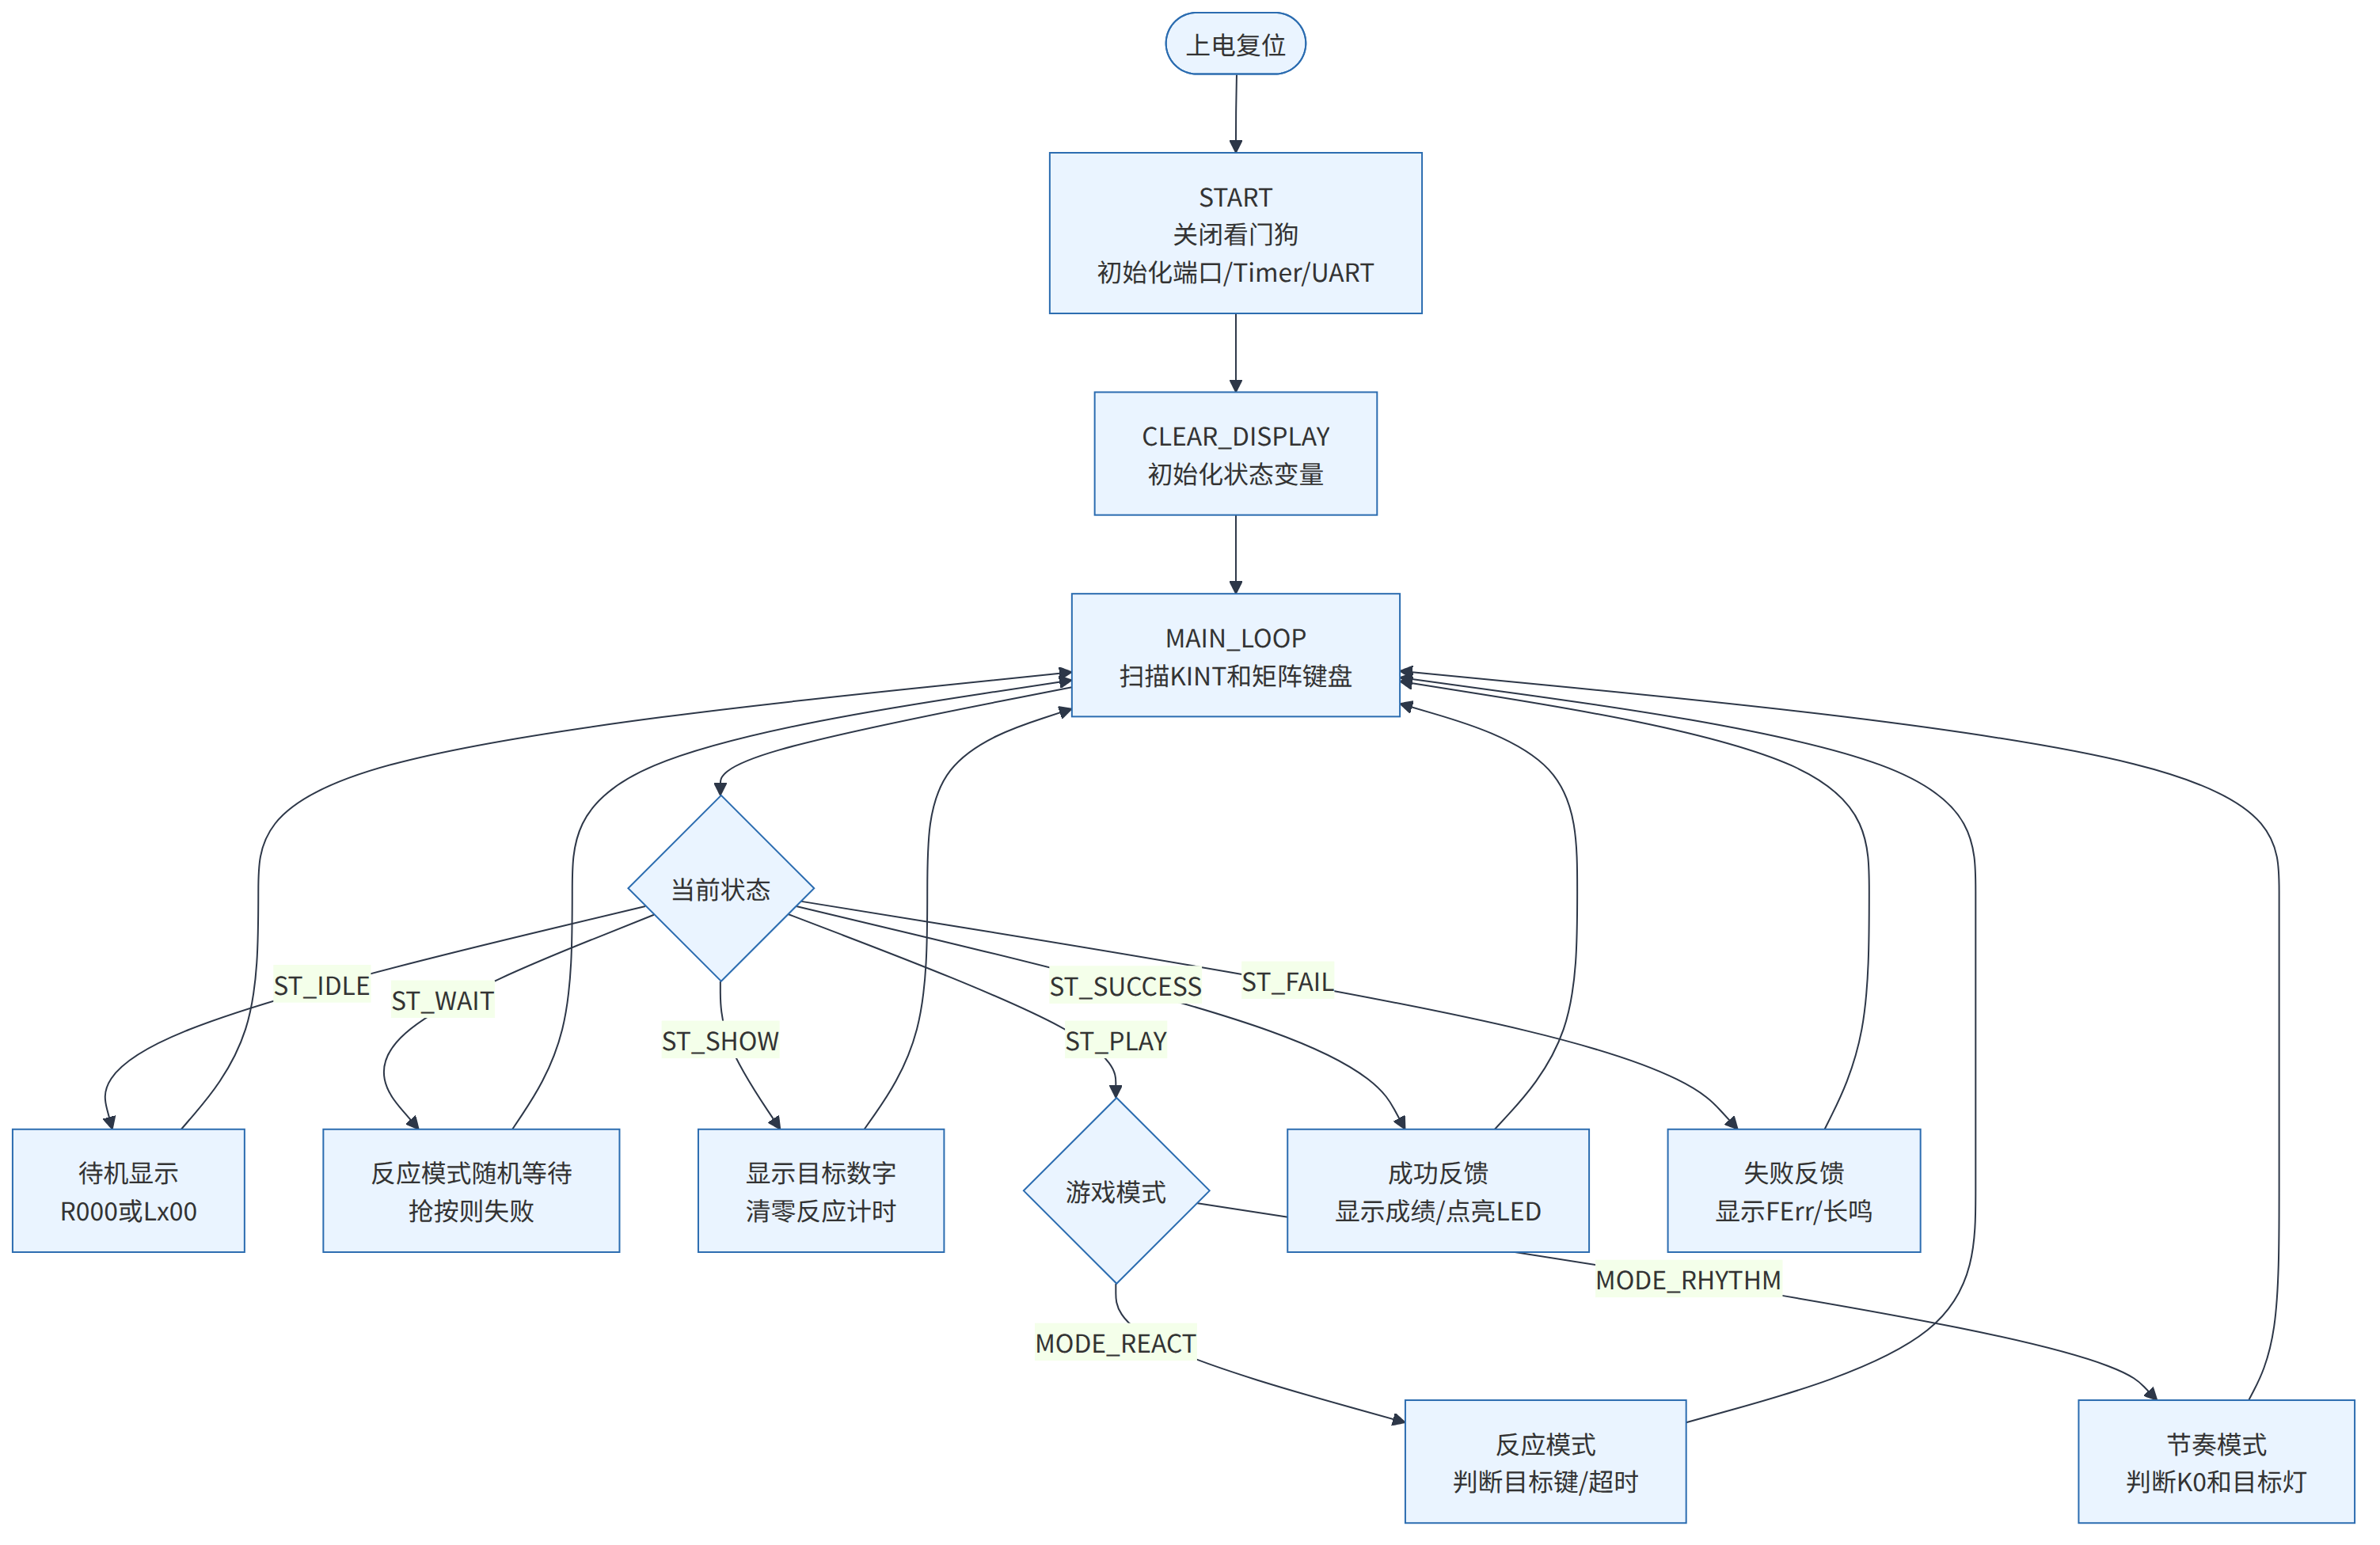
\includegraphics[width=\textwidth,height=0.86\textheight,keepaspectratio]{figures/main_flow.png}
\captionof{figure}{系统软件主流程图}
\end{center}

\begin{center}
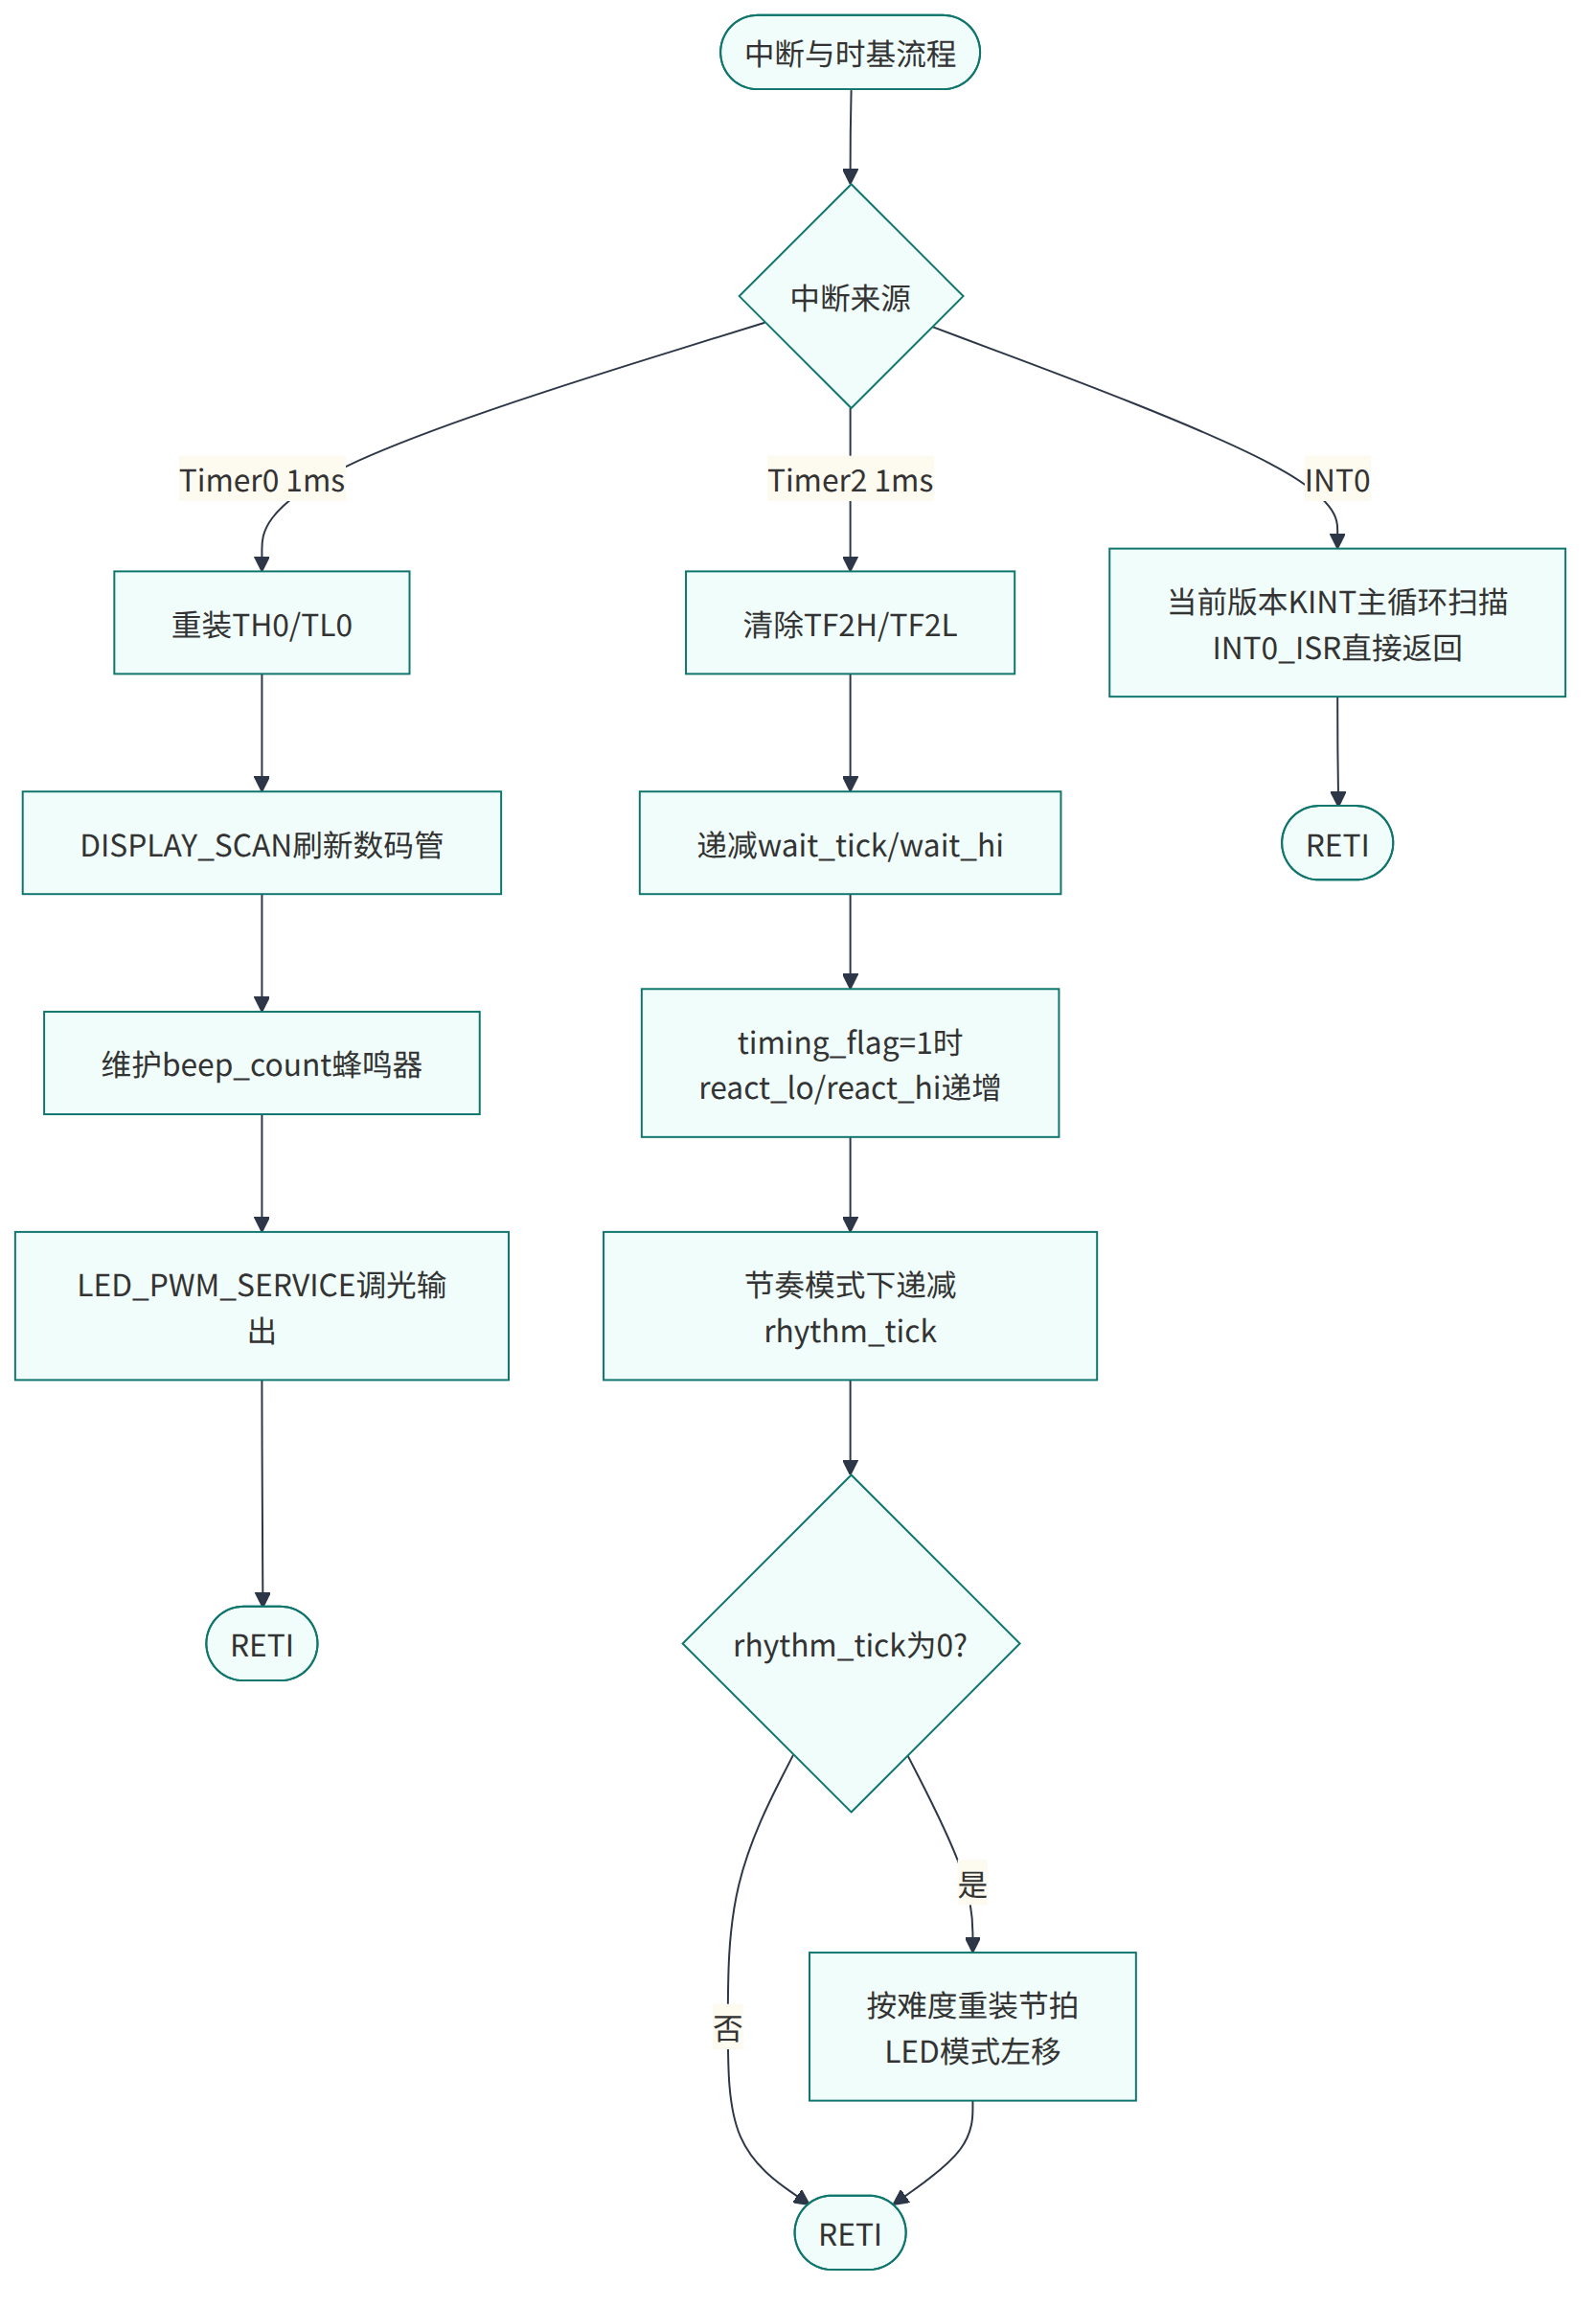
\includegraphics[width=\textwidth,height=0.86\textheight,keepaspectratio]{figures/interrupt_flow.png}
\captionof{figure}{中断与1ms时基流程图}
\end{center}

\subsection{核心算法实现}

\subsubsection*{算法一：随机目标生成与反应时间测量}
本项目的随机数和反应计时均在汇编源代码中直接实现，完整代码见附录\ref{app:code}。轻量级伪随机数由随机数与成绩辅助模块中的MAKE\_RANDOM完成：程序读取历史随机种子，结合Timer0低字节进行异或、循环移位和常数扰动，得到新的\texttt{rand\_seed}。该随机数在游戏逻辑模块中被复用，一方面用于反应模式的随机等待时间，另一方面用于生成0--9目标数字；在节奏模式中，它还用于选择D1--D8目标灯。

反应时间测量的关键流程由游戏逻辑模块中的“显示目标”和“反应作答”两个状态完成。程序在目标数字送入数码管显示变量后，立即调用显示扫描，使目标可见边沿和计时开始尽量同步；随后清零\texttt{react\_lo/react\_hi}并启动Timer2。Timer2的1ms递增逻辑由中断模块维护，当\texttt{timing\_flag}置位时持续累计16位反应时间。玩家按键后，主循环先锁存第一次扫描到的反应时间，再做消抖确认，因此消抖延时不会被计入最终成绩。反应时间转4位十进制显示由显示模块完成，相关代码均见附录\ref{app:code}。

\subsubsection*{算法二：矩阵键盘扫描、消抖与节奏命中判定}
矩阵键盘使用P2口。P2.0--P2.3作为行扫描输出，对应KO.0--KO.3；P2.4--P2.7作为列输入，对应KI.0--KI.3。程序每次把一行拉低，其余行置高，然后读取高四位列输入。如果某一列读到低电平，说明当前行列交点按键被按下。根据实验板按键示意图，内部键值采用“键值=列号×4+行号”的规则：第一列从上到下为K0、K1、K2、K3，第二列为K4--K7，第三列为K8--K11，第四列为K12--K15。

节奏挑战模式在开始时随机确定一个目标灯D1--D8，数码管显示为\texttt{LxSS}，其中x是目标灯编号，SS是分数。玩家只有在目标灯亮起时按K0才得分；K10、K11、K12用于低、中、高三档速度设置；K15用于模式切换。三档难度均为单灯命中，区别是流水灯步进周期不同：低难度约220ms/步，中难度约160ms/步，高难度约90ms/步。节奏模式达到20分判定成功。

矩阵键盘扫描、消抖和按键释放等待均由键盘模块实现，完整代码见附录\ref{app:code}。其中SCAN\_KEY\_RAW负责逐行拉低P2.0--P2.3并读取P2.4--P2.7列输入，SCAN\_KEY在原始键值基础上加入软件消抖，WAIT\_MATRIX\_RELEASE用于防止一次长按被重复计入。KINT独立按键同样通过SCAN\_KINT完成稳定按下和释放检测。

节奏命中判定由游戏逻辑模块中的STATE\_RHYTHM\_PLAY完成。程序要求玩家按下K0，并且当前\texttt{led\_pattern}必须等于目标灯模式\texttt{rhythm\_pat}，两者同时满足才增加\texttt{rhythm\_score}。LED目标表由查找表模块提供；流水灯输出和软件PWM调光由LED模块完成；节奏速度控制由中断模块中的Timer2分支维护。低、中、高三档难度的步进周期分别约为220ms、160ms和90ms，最终由\texttt{rhythm\_tick}的重装值体现。上述实现对应的完整代码见附录\ref{app:code}。

\section{作品创新点和人机交互设计}

\subsection{创新点阐述}
\textbf{创新点一：双模式挑战与键盘难度设置。}普通反应力小游戏通常只有单一玩法，本项目在同一块C8051F310开发板上实现反应力测试和节奏挑战两种模式。K15用于模式切换，K10--K12用于节奏模式低、中、高三档速度设置。与固定速度的单一游戏相比，本作品既能测量反应时间，也能训练节奏感和手眼协调能力。该创新点使用状态机、矩阵键盘功能键分配、Timer2节拍控制和数码管模式显示实现。

\textbf{创新点二：多模态声光反馈。}本项目不是单纯用数码管显示数字，而是把数码管、LED流水灯和蜂鸣器组合为完整反馈系统。数码管负责显示分数、时间和目标键；LED负责倒计时、节奏移动和成功动画；蜂鸣器负责开始、成功、失败和超时提示。与单一显示产品相比，用户无需阅读说明即可理解当前状态，现场演示效果更强。

\textbf{创新点三：准确计时与柔和LED显示。}反应模式不是简单在按键消抖后读取时间，而是在目标数字显示到数码管端口后立即启动Timer2，并在第一次扫描到按键时锁存16位反应时间，误差控制在10ms以内。LED流水灯通过74HCT164串行输出，同时加入软件PWM调光，使现场演示时灯光更柔和。该创新点使用Timer2自动重装载、16位时间变量、二进制转BCD显示和LED占空比控制实现。

\subsection{人机交互设计}
本作品实现三种主要交互方式。

第一种是矩阵键盘交互。用户可通过4x4键盘参与挑战，其中K0--K9用于反应模式数字目标输入，K0也作为节奏模式命中键；K10、K11、K12分别设置节奏模式低、中、高难度；K15用于反应模式和节奏模式切换。系统检测到有效按键后，蜂鸣器短响，数码管更新显示，保证用户获得即时反馈。

第二种是外部触发键交互。P0.1独立触发键KINT作为快速开始/下一轮按键，按下时为低电平。现场演示时，体验者只需按一下KINT即可开始当前模式；成功或失败后结果保持在数码管上，再次按KINT进入下一轮，提高了演示效率。

第三种是声光反馈交互。数码管显示当前模式、目标数字、目标灯编号、分数、反应时间或\texttt{FErr}错误提示；LED流水灯显示等待动画和节奏进度；蜂鸣器用短响、长响区分开始、成功和失败。演示者可以先展示低难度，再切换高难度，让观众直接看到LED节奏加快。

\begin{center}
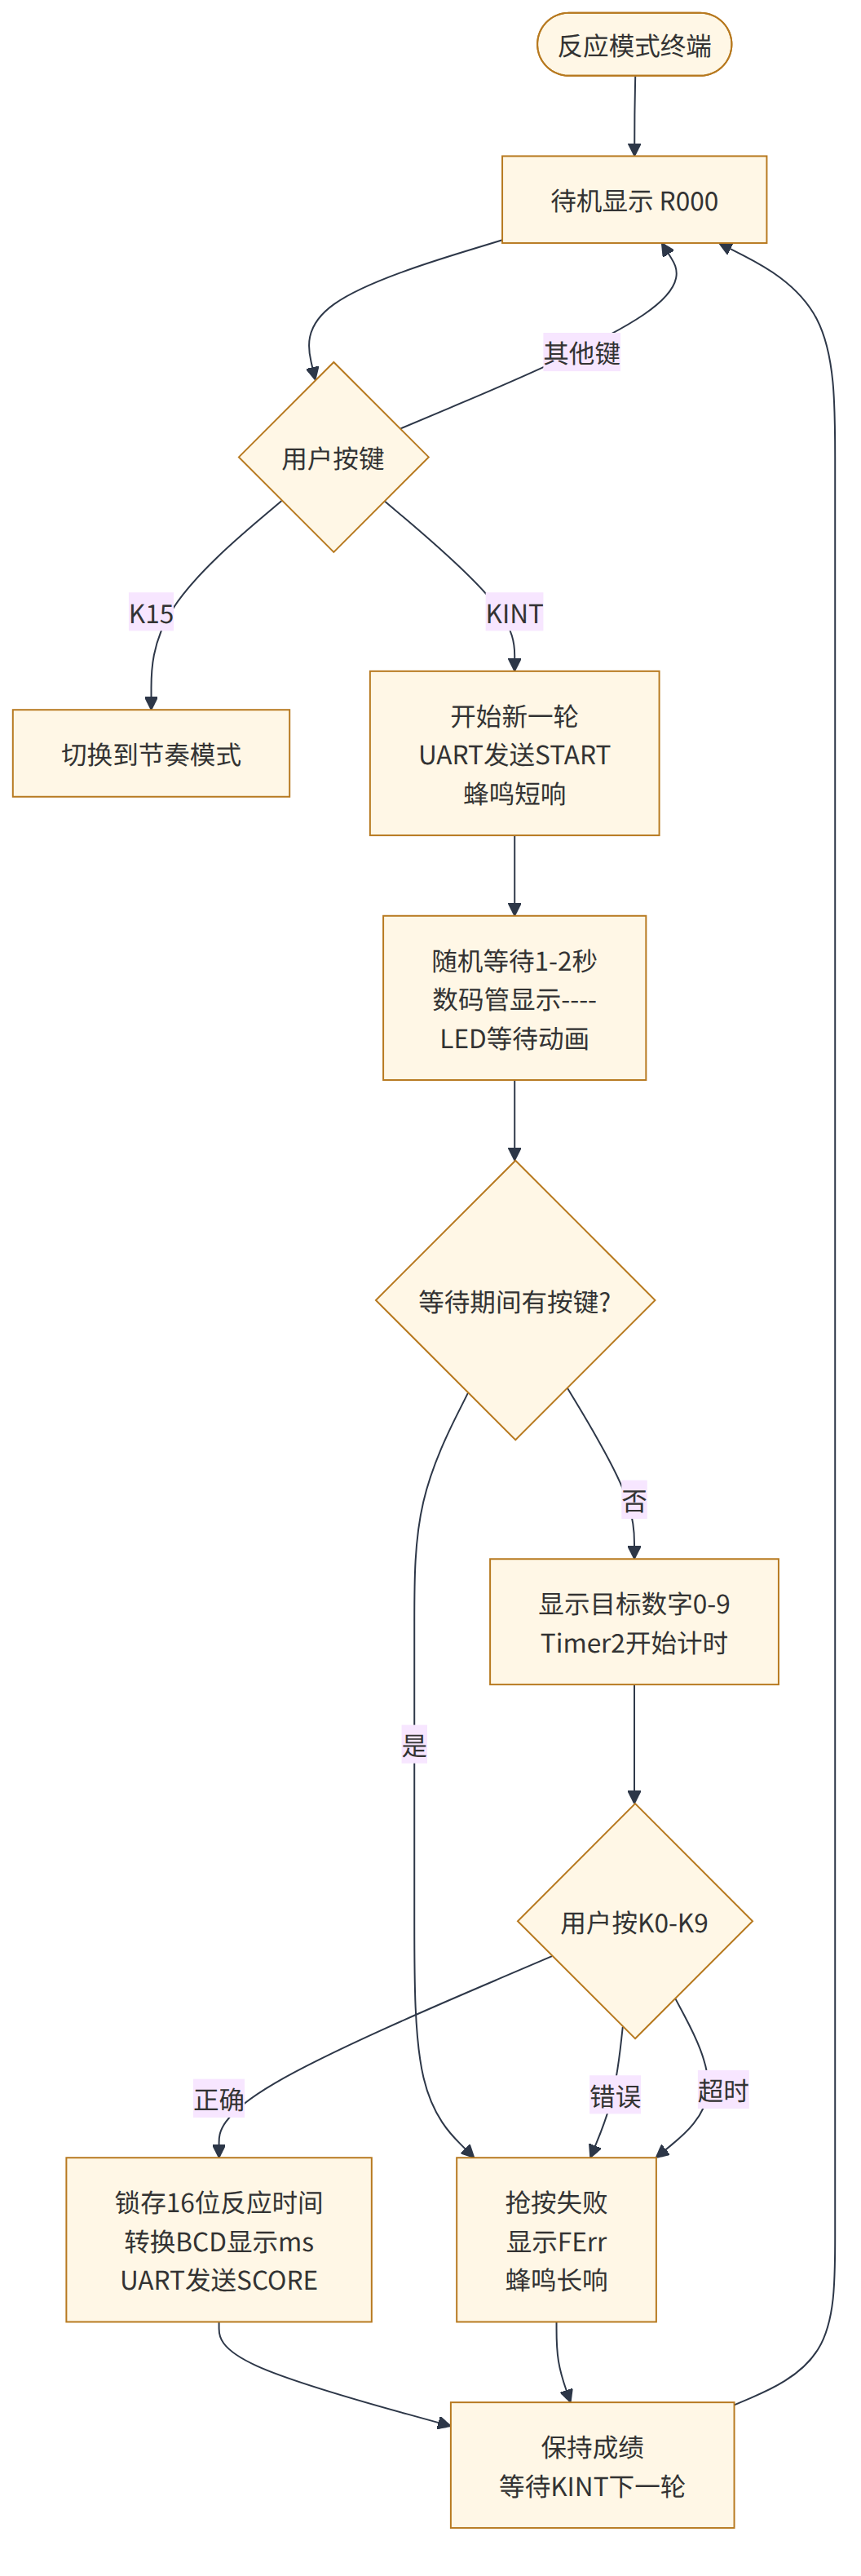
\includegraphics[width=\textwidth,height=0.86\textheight,keepaspectratio]{figures/reaction_terminal_flow.png}
\captionof{figure}{反应模式终端流程图}
\end{center}

\begin{center}
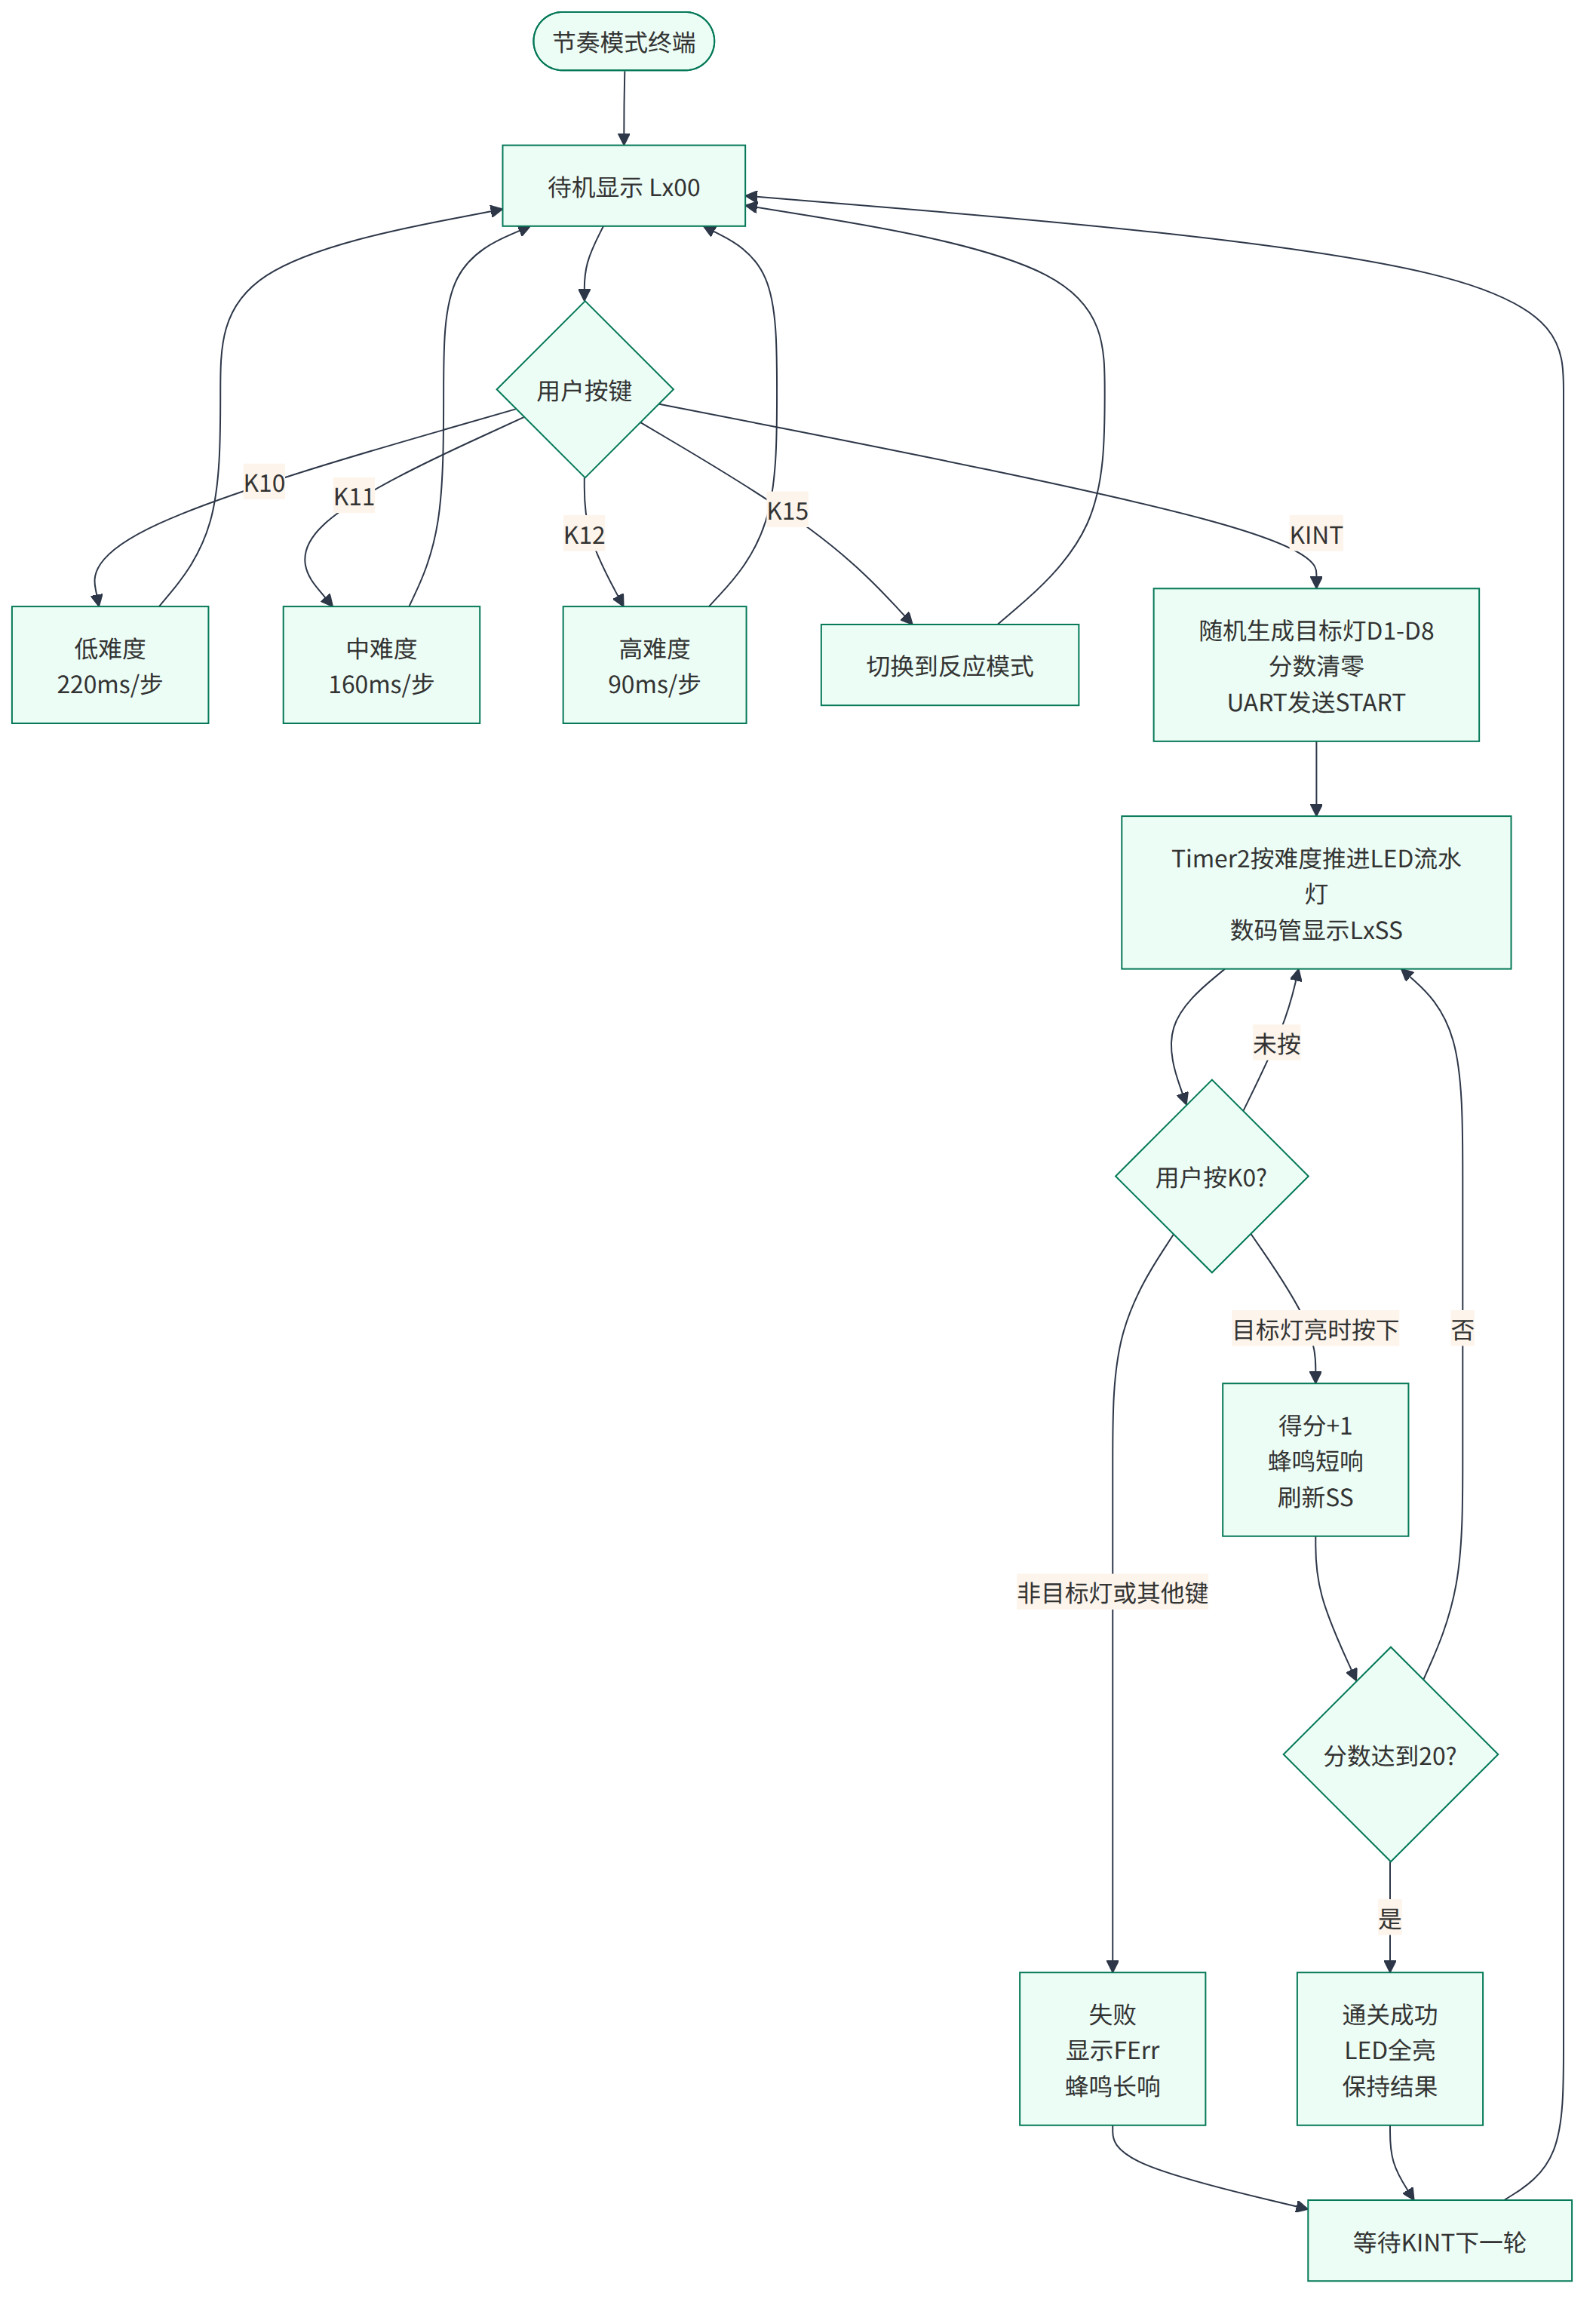
\includegraphics[width=\textwidth,height=0.86\textheight,keepaspectratio]{figures/rhythm_terminal_flow.png}
\captionof{figure}{节奏模式终端流程图}
\end{center}

\begin{center}
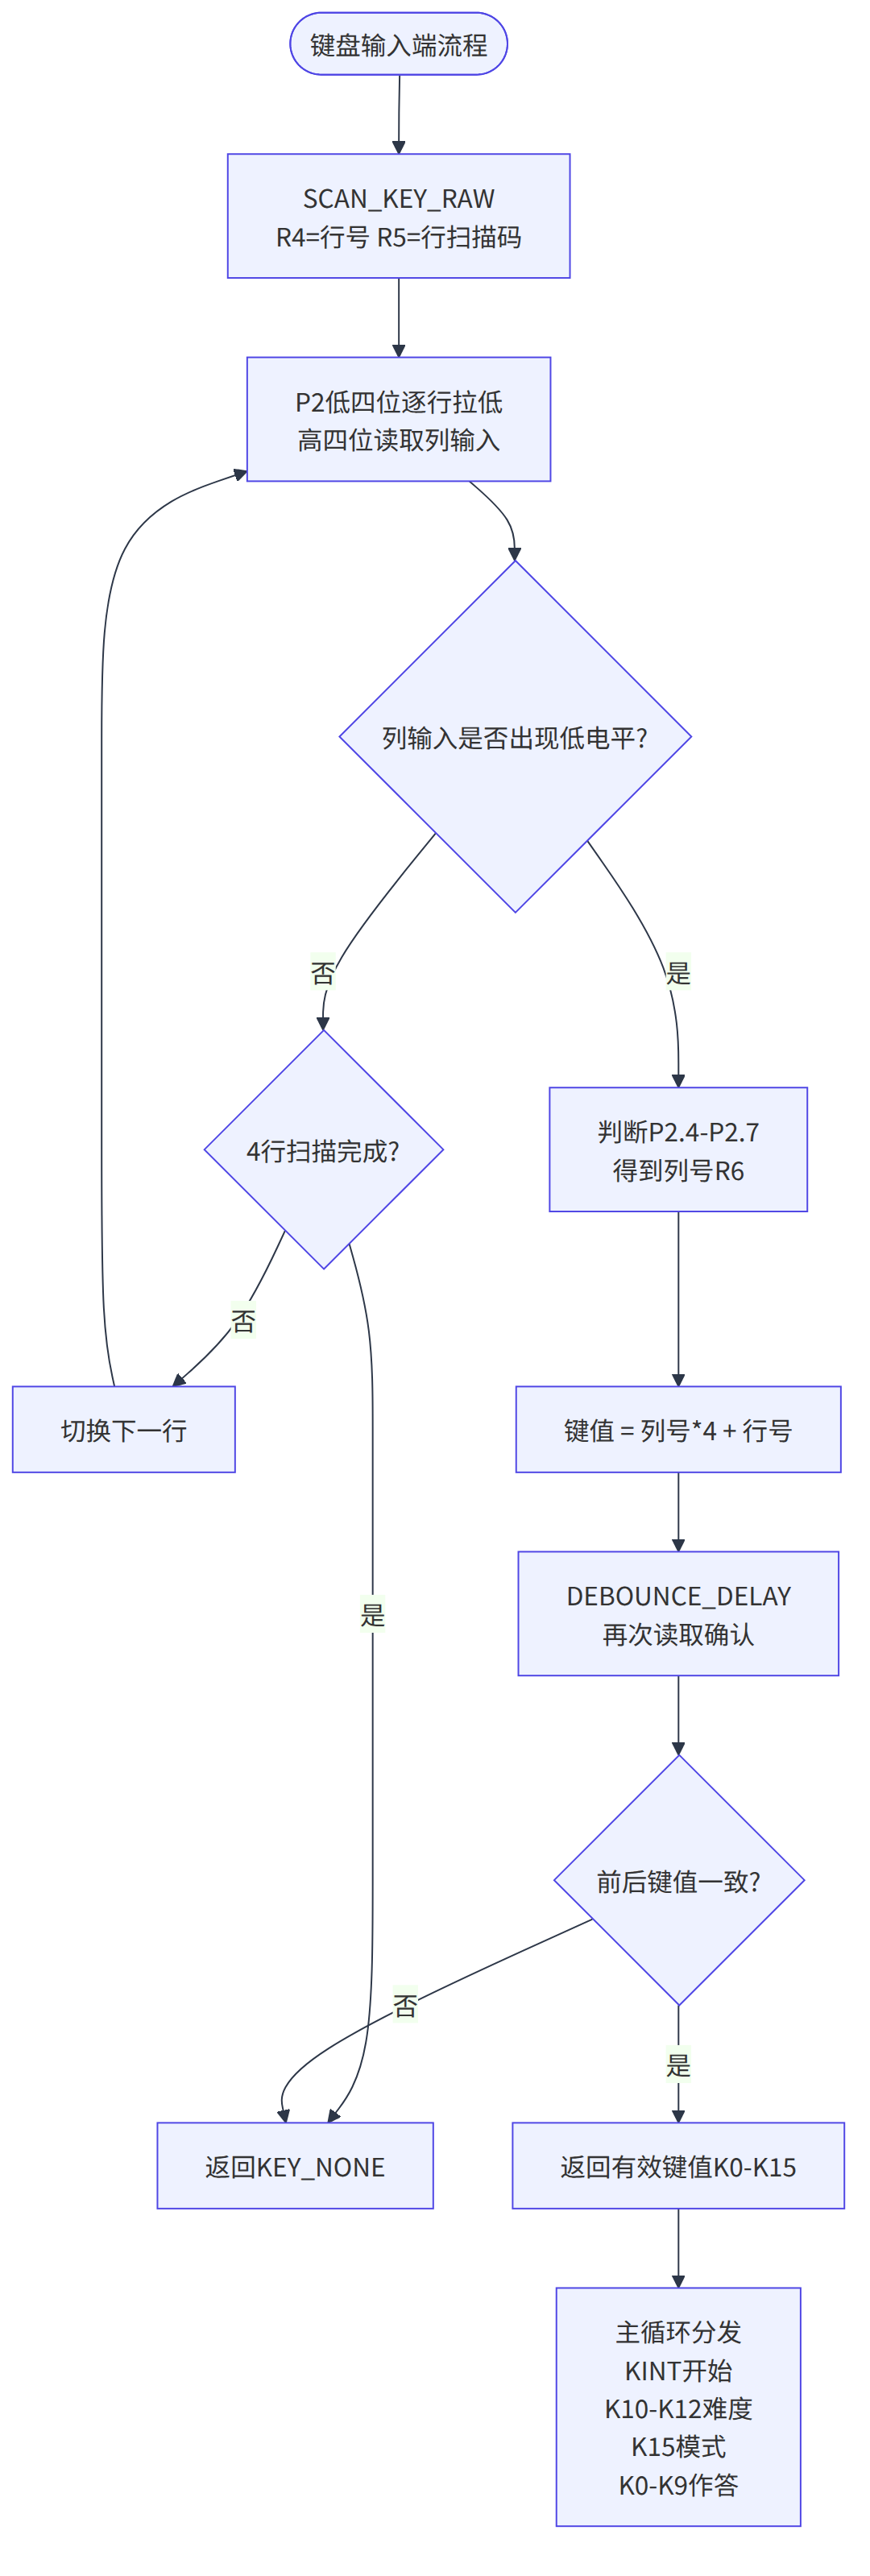
\includegraphics[width=\textwidth,height=0.86\textheight,keepaspectratio]{figures/keypad_terminal_flow.png}
\captionof{figure}{键盘输入端流程图}
\end{center}

\begin{center}
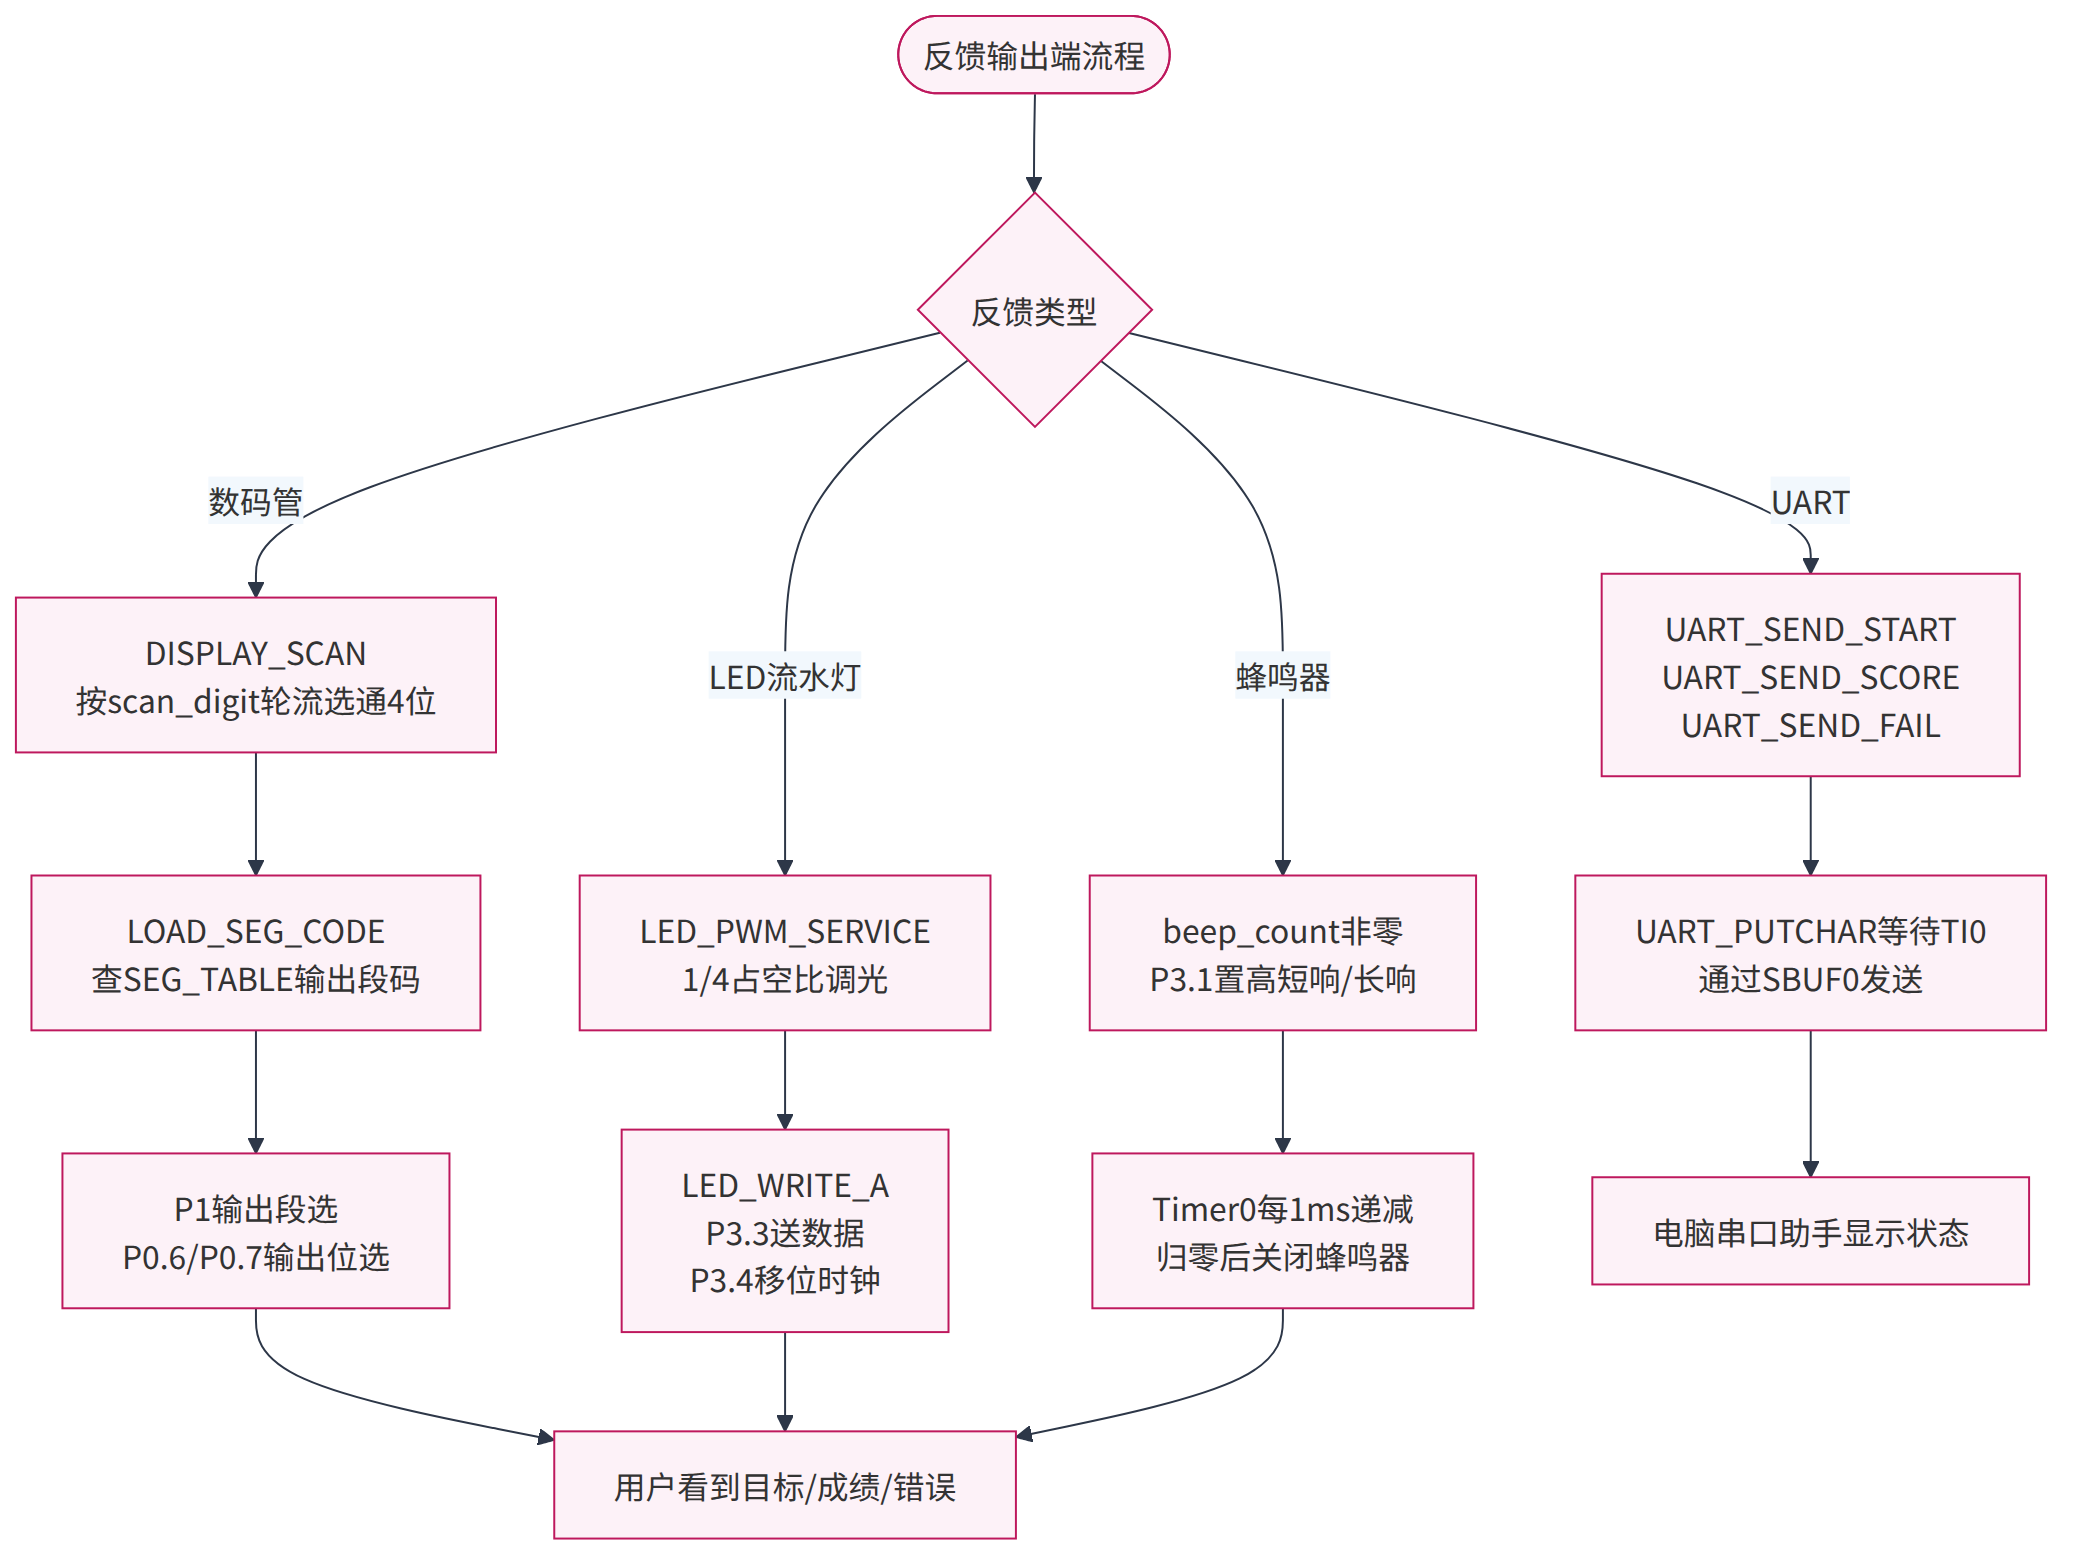
\includegraphics[width=\textwidth,height=0.86\textheight,keepaspectratio]{figures/feedback_terminal_flow.png}
\captionof{figure}{反馈输出端流程图}
\end{center}

现场演示中，演示者先说明规则，然后让观众按K15选择模式。反应模式下，观众按KINT开始，数码管随机显示0--9中的目标数字，观众按对应K0--K9数字键作答；成功时蜂鸣器短响并显示反应时间，失败时蜂鸣器长响并显示\texttt{FErr}。节奏模式下，观众先用K10--K12选择难度，再按KINT开始；数码管显示\texttt{LxSS}，其中x为本局随机目标灯编号，观众在对应LED亮起时按K0得分，达到20分通关。

\section{小组讨论发言}

按照模板要求，本节记录不少于6次小组讨论。由于聊天截图尺寸较大，采用分小节记录的方式，每次讨论单独说明主题、发言要点、形成结论，并插入对应截图。

\subsection{第一次讨论：项目选题比较}
组长提出密码锁、抢答器、番茄钟、反应力游戏等候选方案。组员讨论后认为，科创集市作品需要具备现场互动性、可竞争性和直观反馈效果，因此最终确定“反应力与节奏挑战训练仪”作为项目主题。

\begin{center}
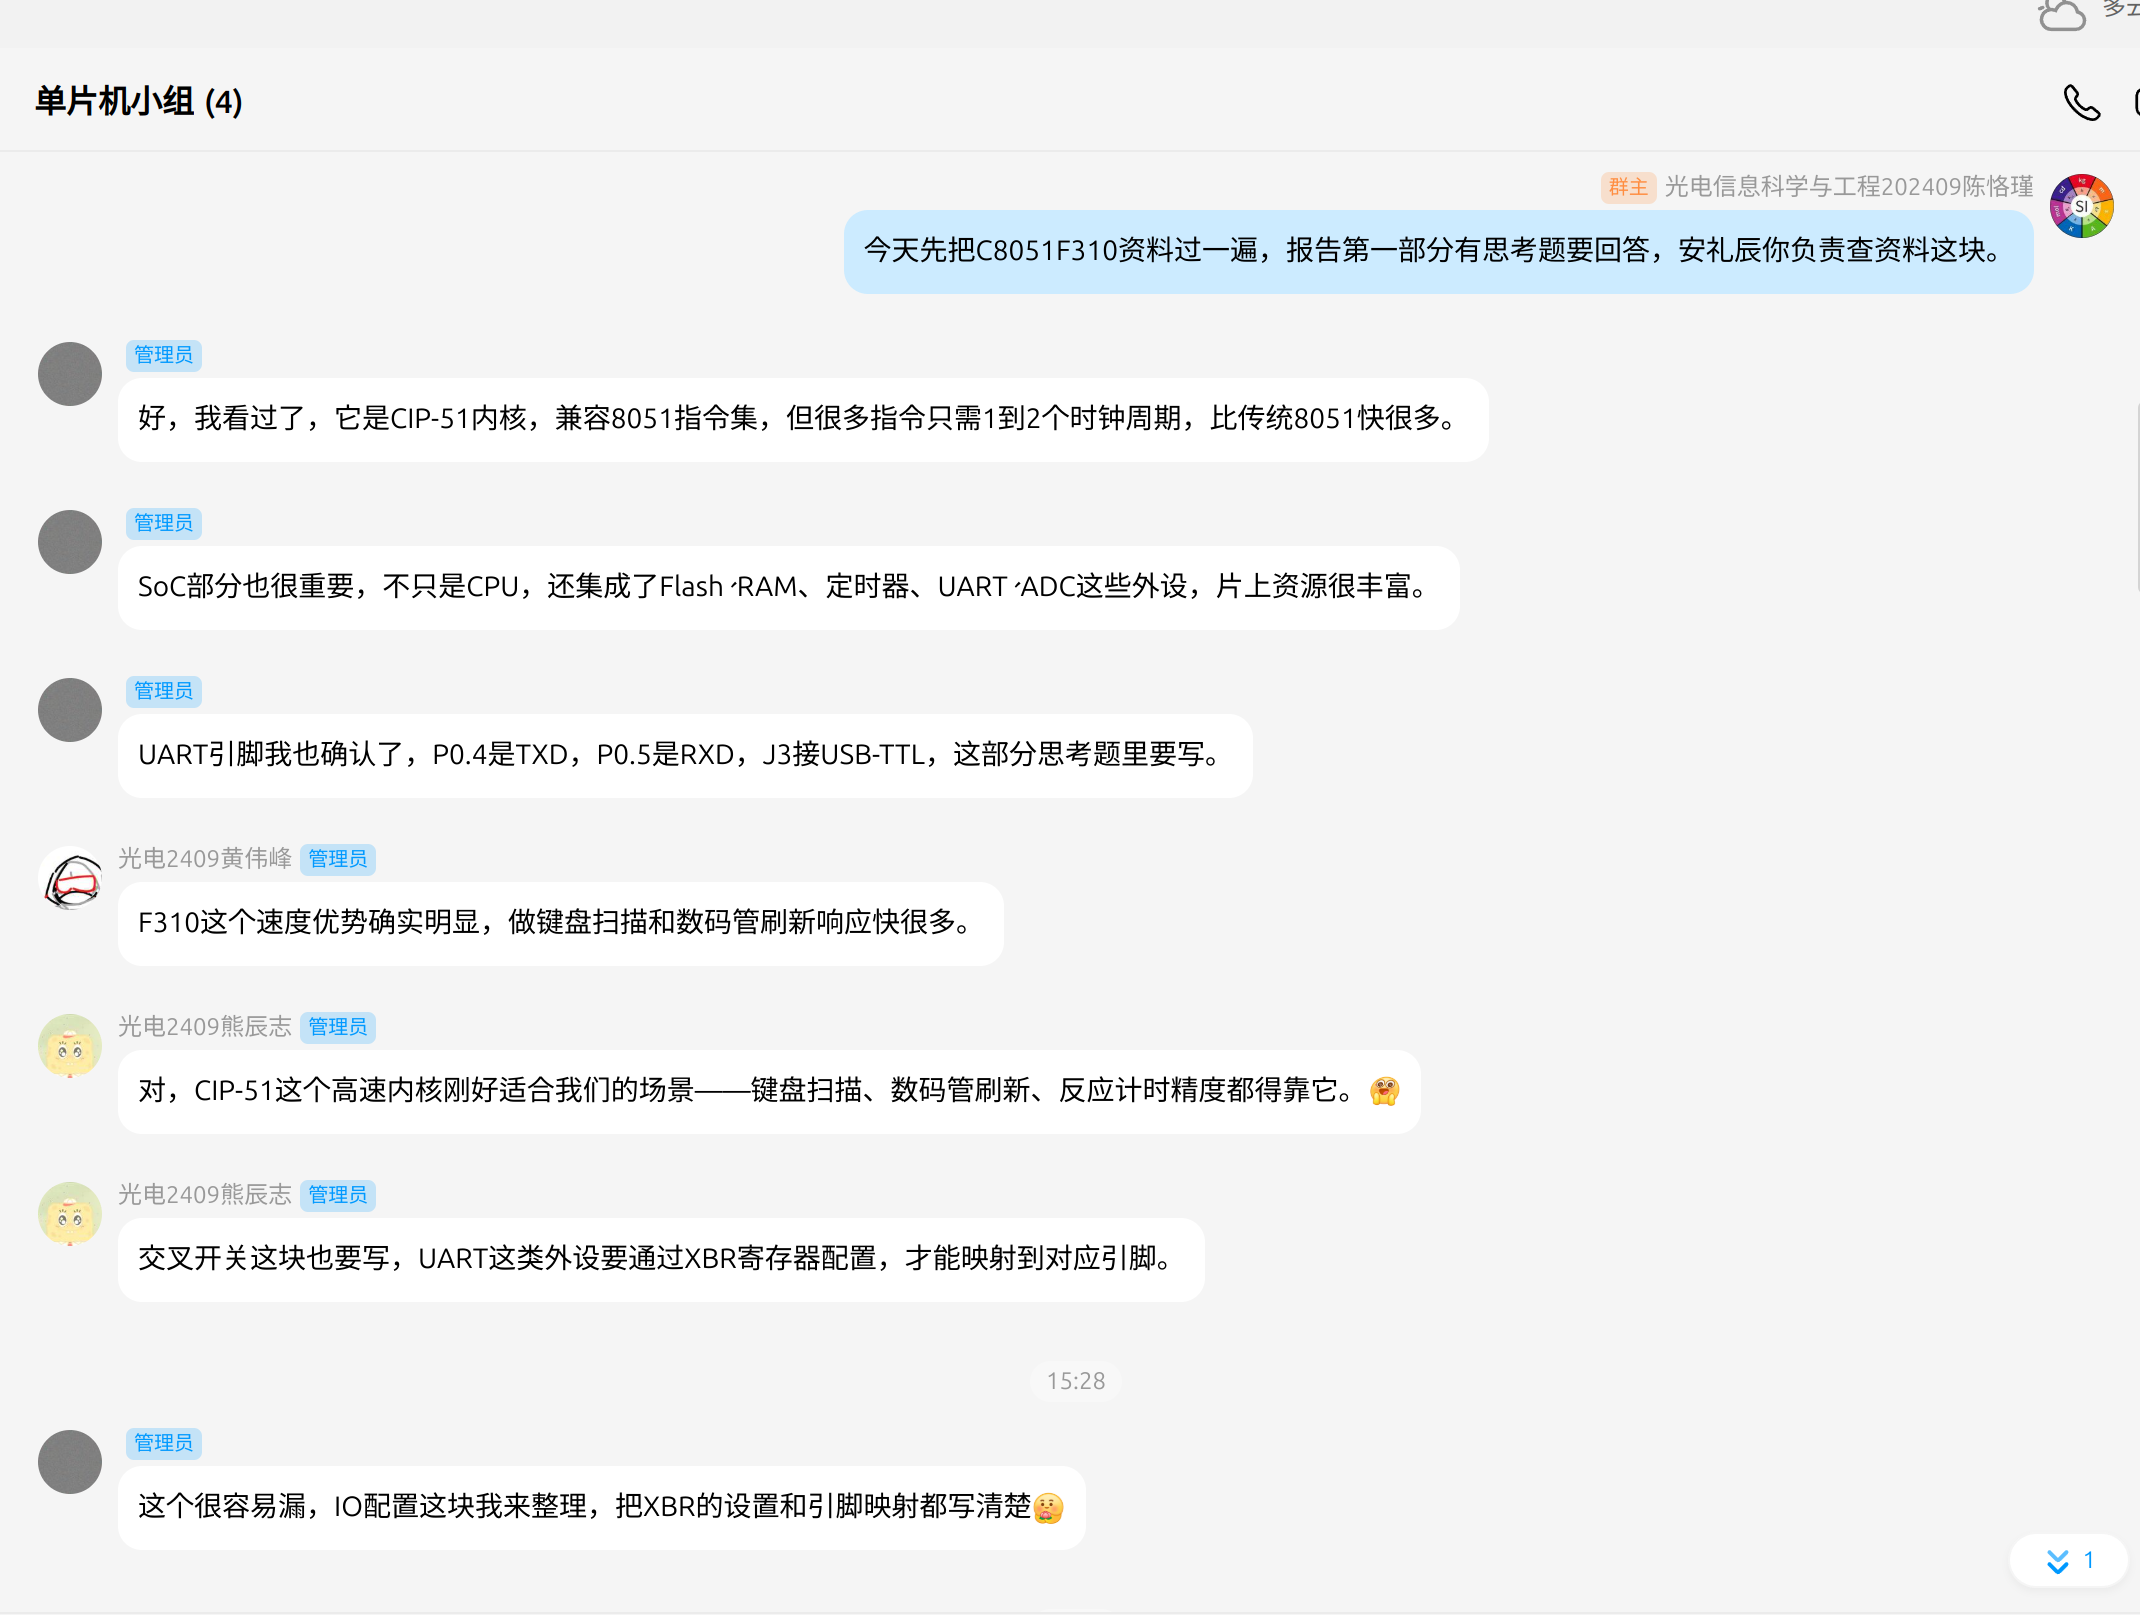
\includegraphics[width=\textwidth,height=0.82\textheight,keepaspectratio]{figures/screenshots/1-1.png}
\captionof{figure}{第一次讨论截图1}
\end{center}

\begin{center}
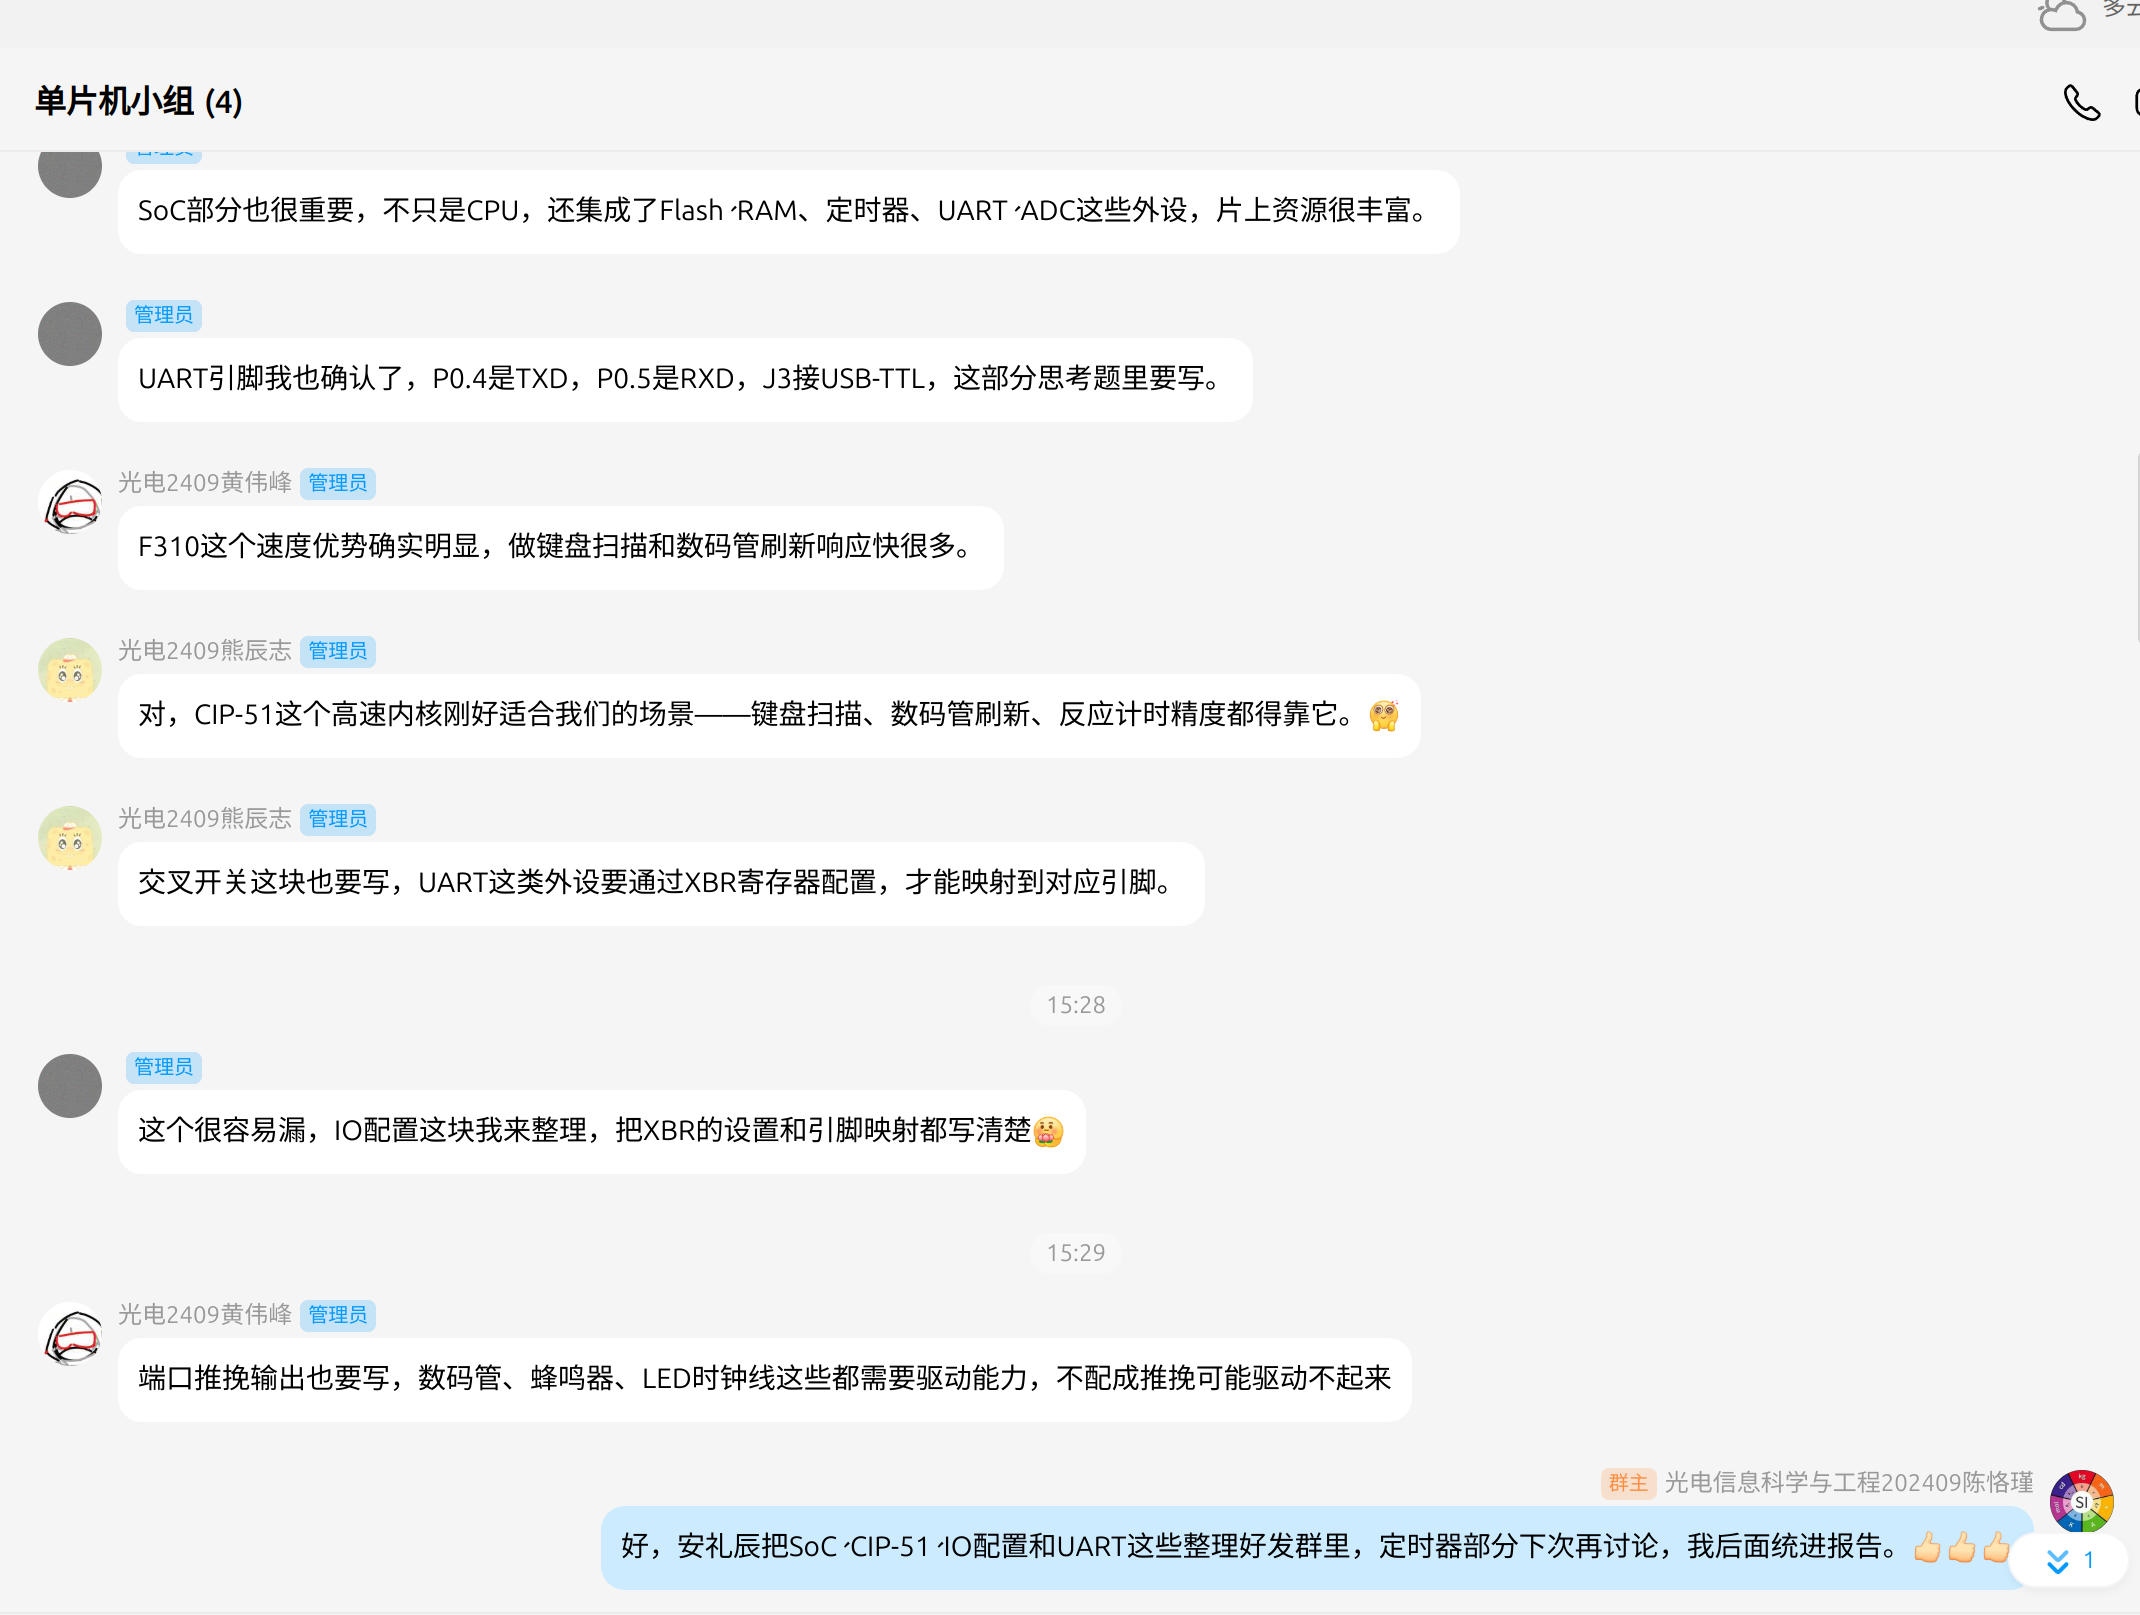
\includegraphics[width=\textwidth,height=0.82\textheight,keepaspectratio]{figures/screenshots/1-2.png}
\captionof{figure}{第一次讨论截图2}
\end{center}

\subsection{第二次讨论：C8051F310资料学习}
本次讨论围绕C8051F310新特性、CIP-51内核、SoC集成资源、定时器时钟、交叉开关和UART接口展开。讨论结论是项目应尽量覆盖开发板上的数码管、矩阵键盘、LED流水灯、蜂鸣器、KINT按键和串口资源。

\begin{center}
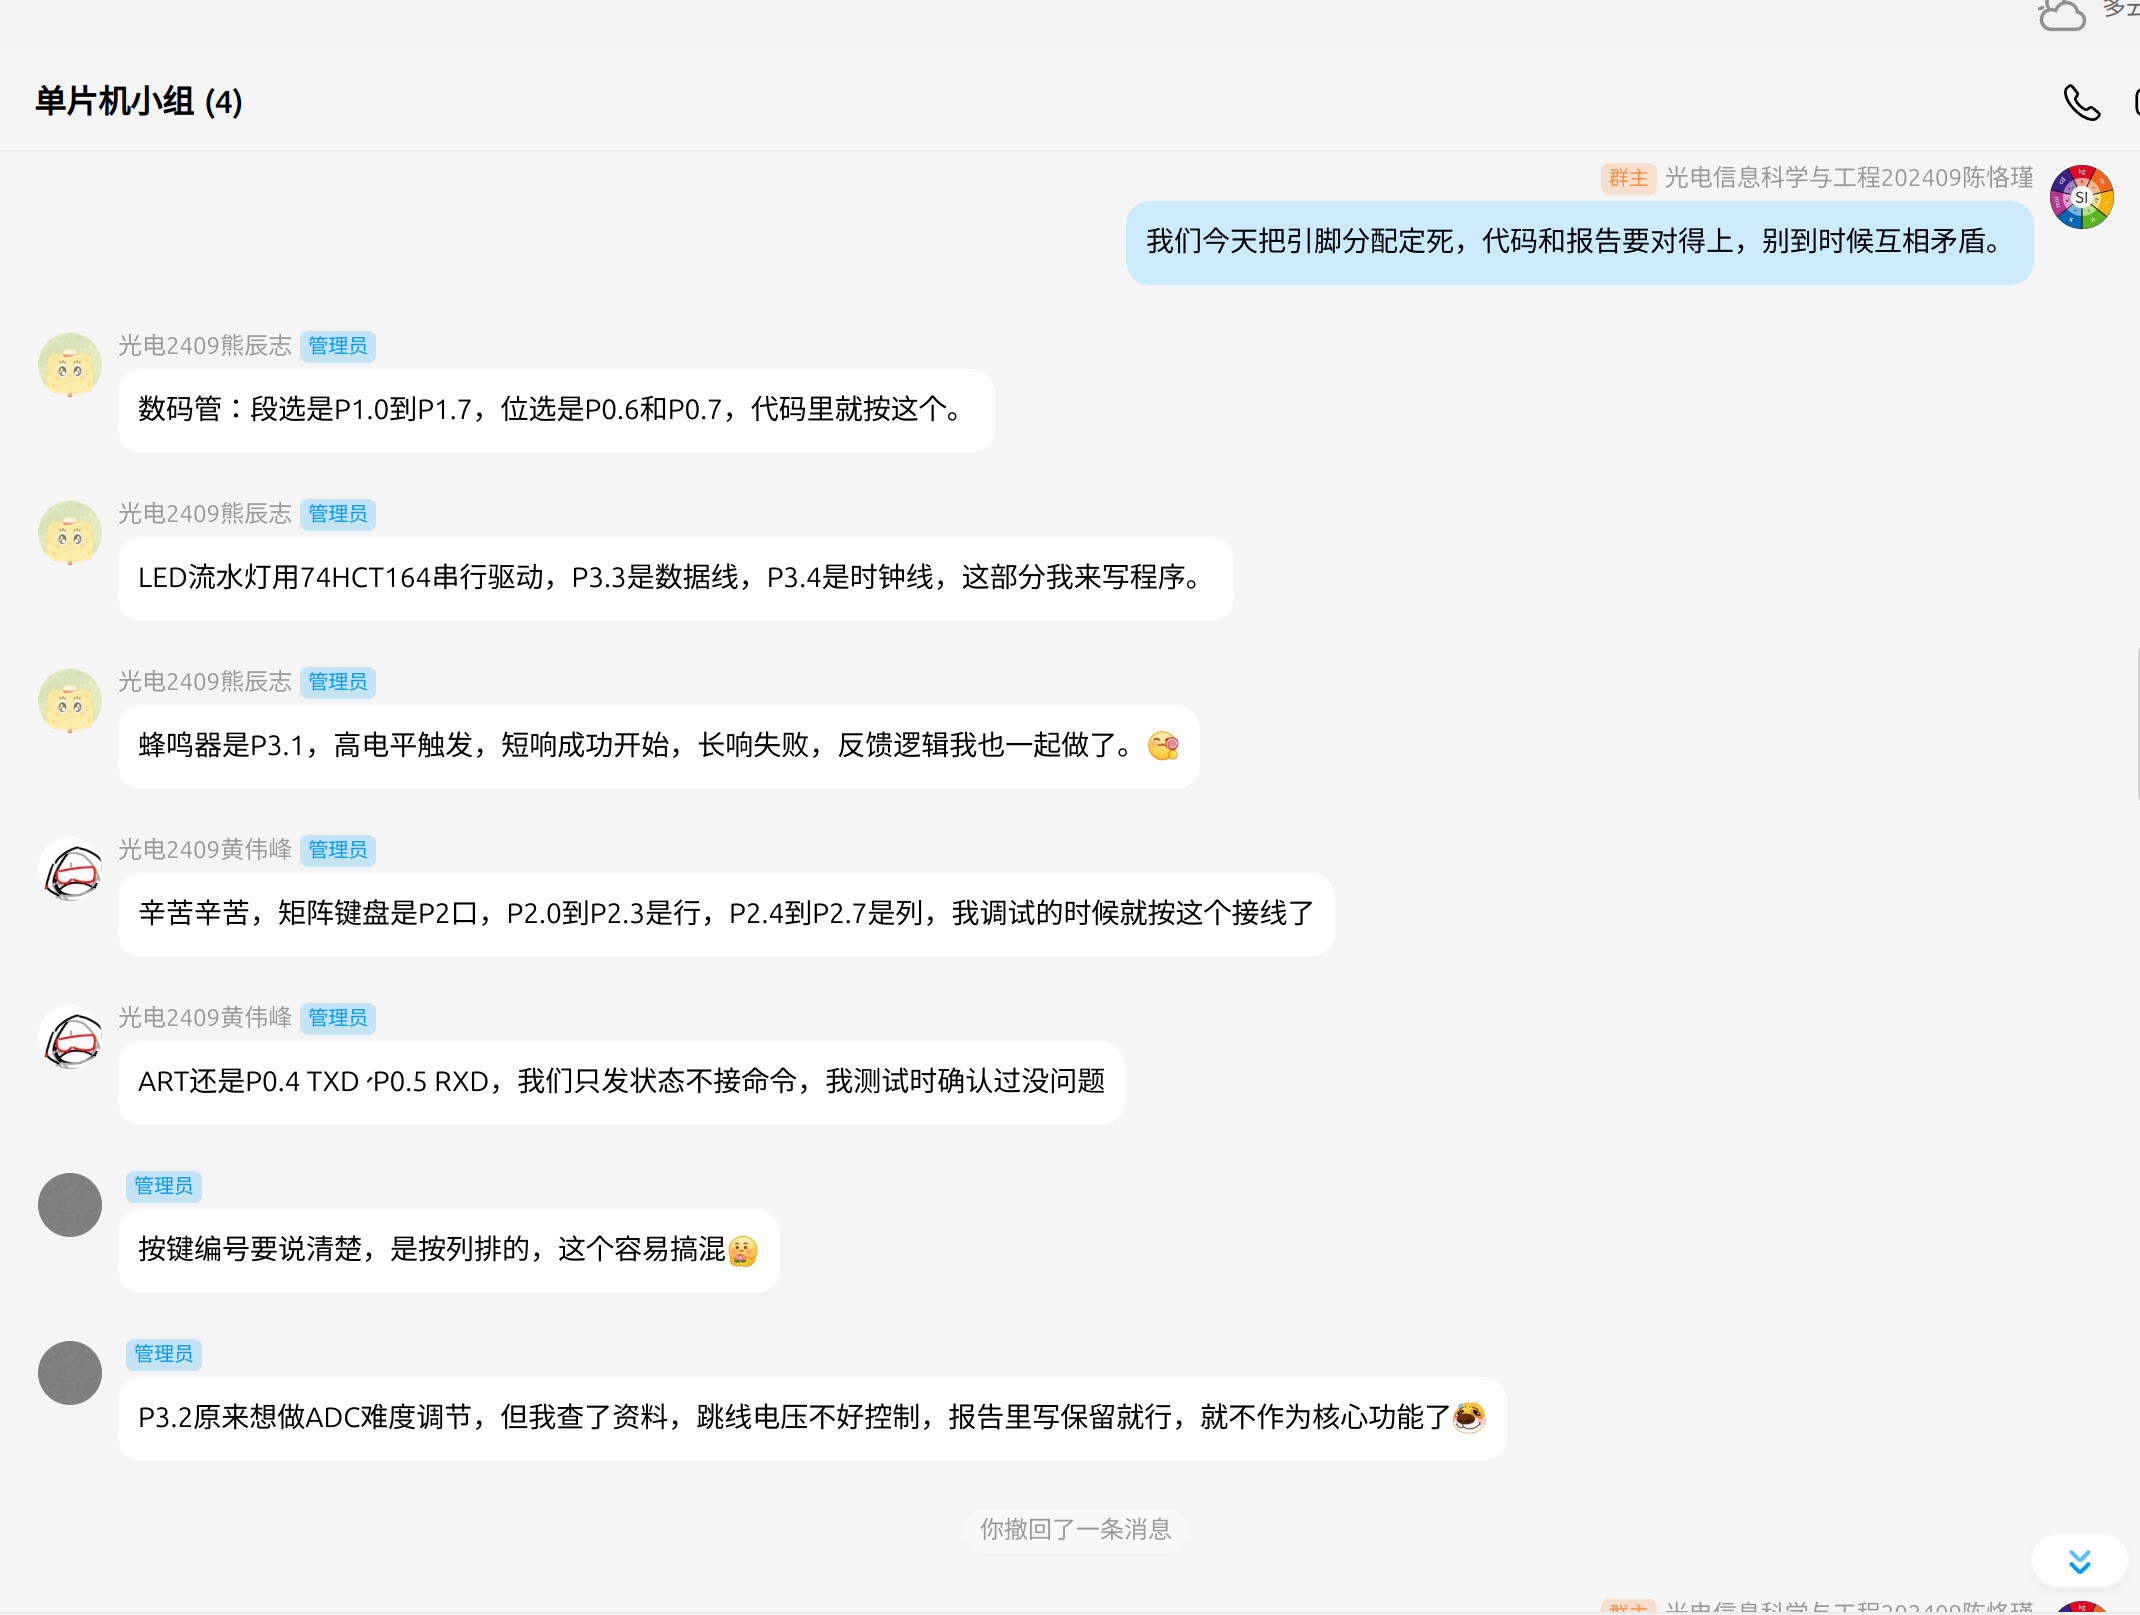
\includegraphics[width=\textwidth,height=0.82\textheight,keepaspectratio]{figures/screenshots/2-1.png}
\captionof{figure}{第二次讨论截图1}
\end{center}

\begin{center}
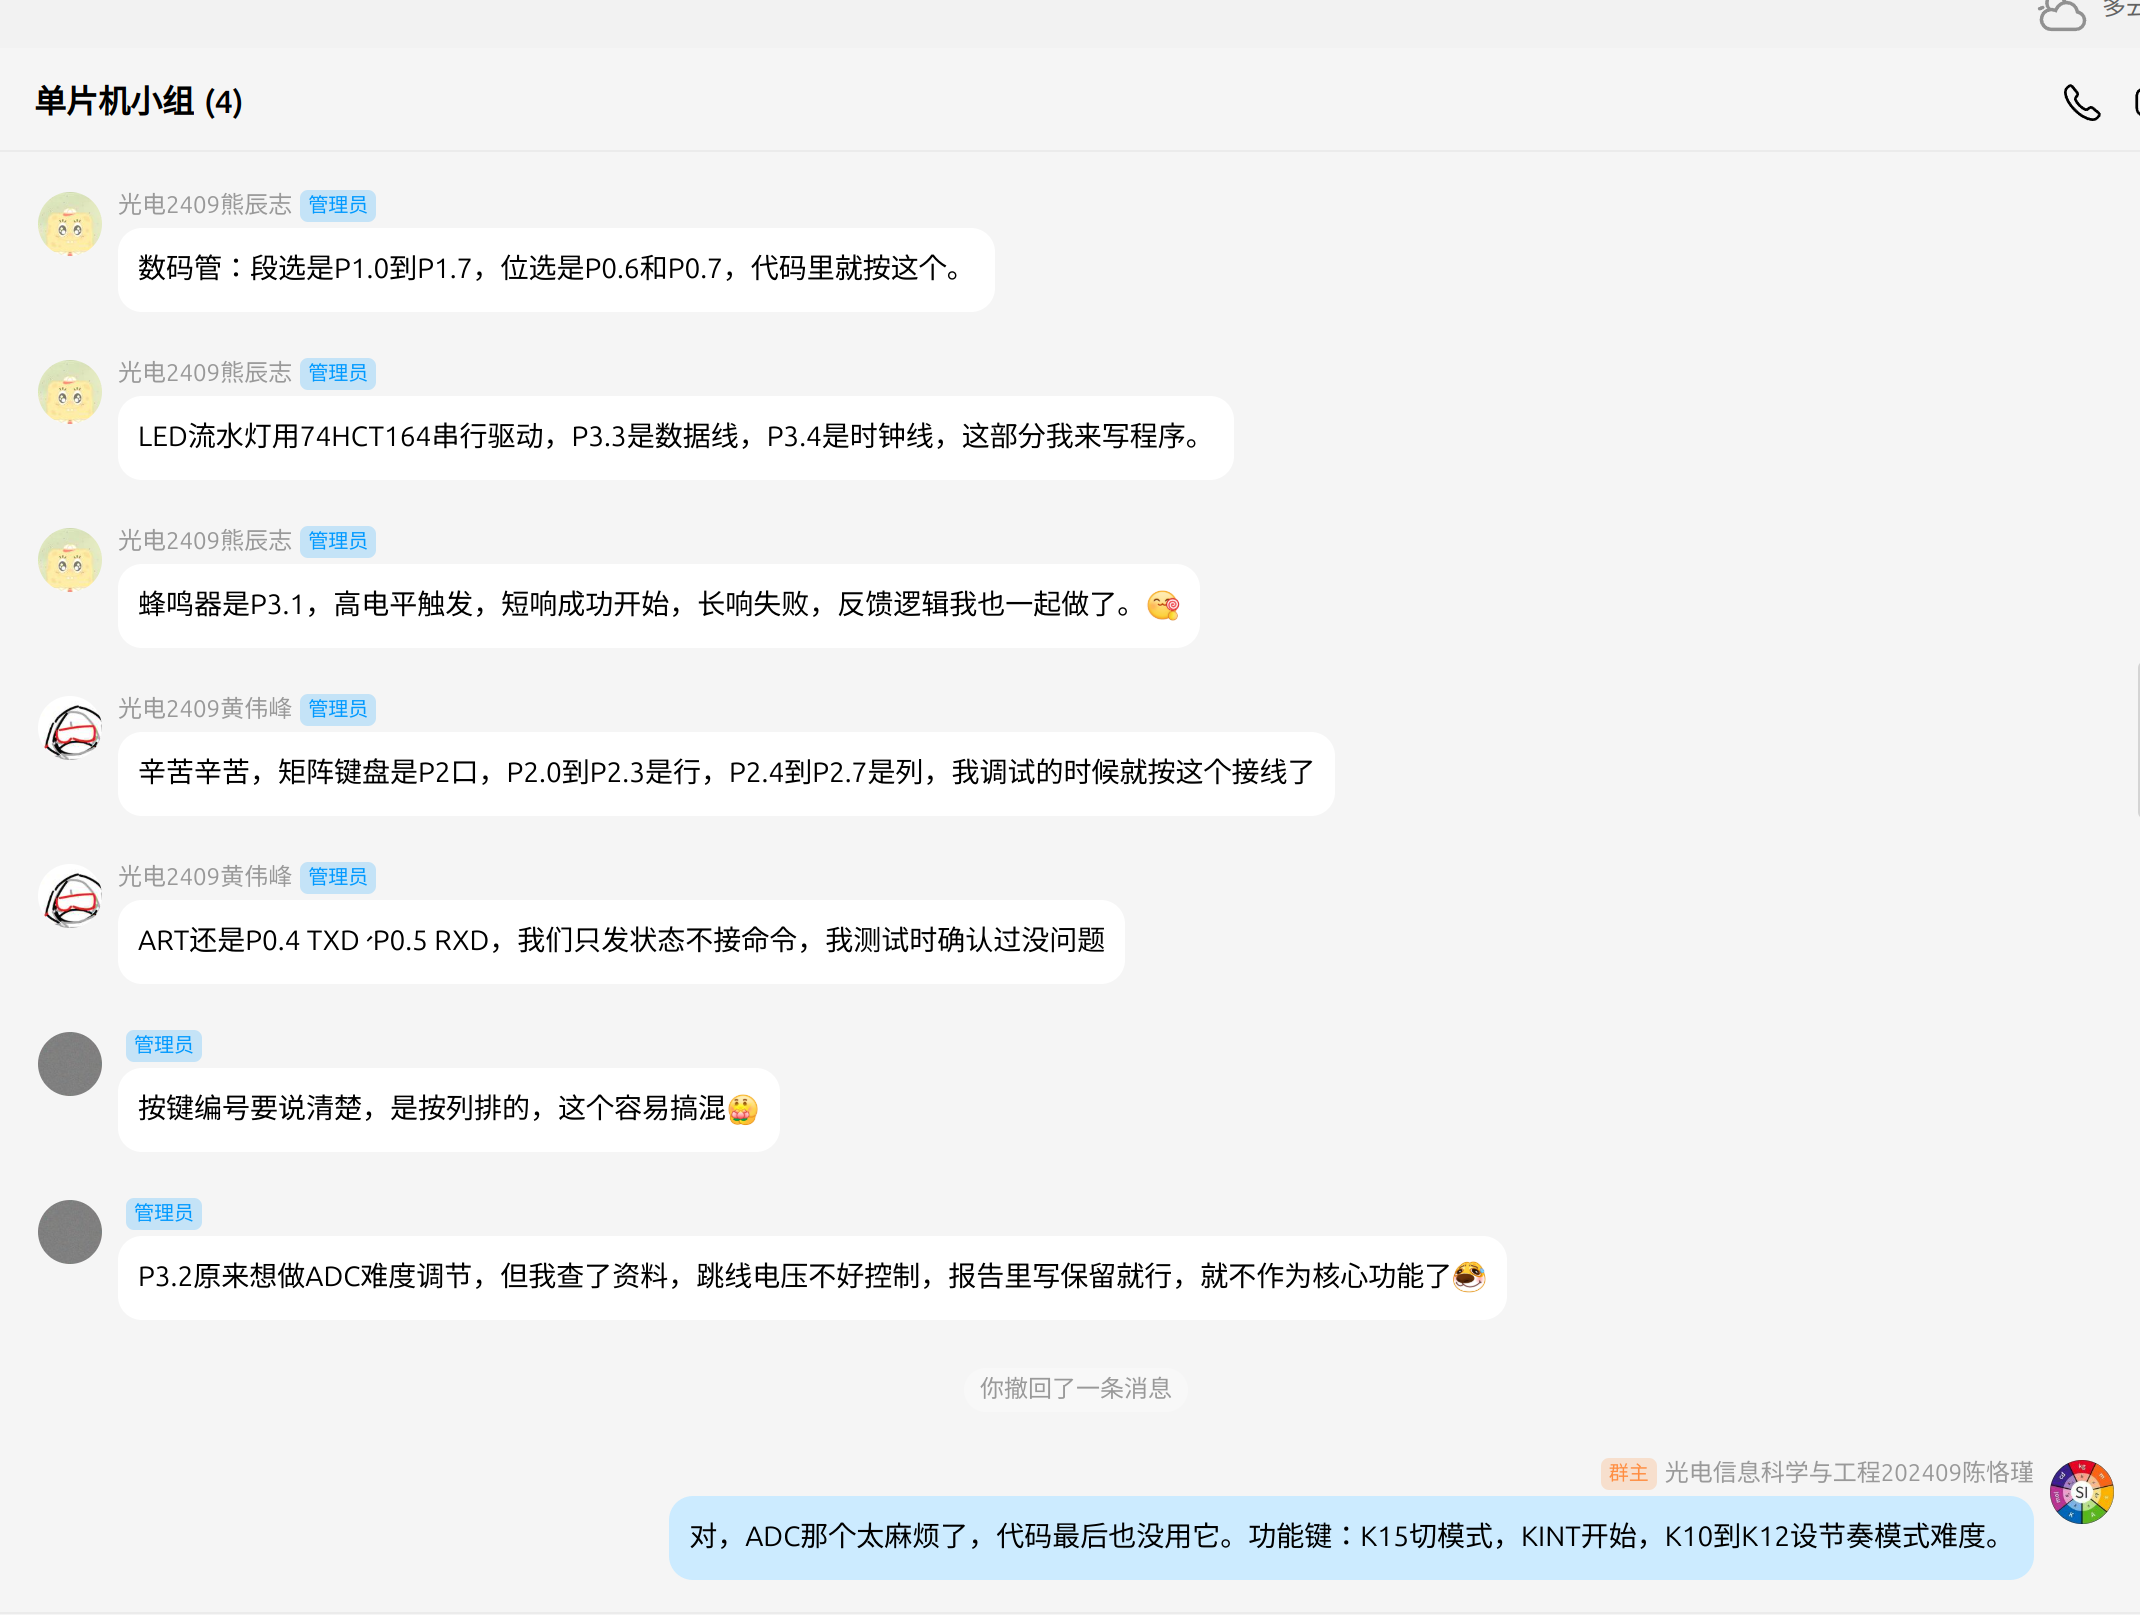
\includegraphics[width=\textwidth,height=0.82\textheight,keepaspectratio]{figures/screenshots/2-2.png}
\captionof{figure}{第二次讨论截图2}
\end{center}

\subsection{第三次讨论：硬件资源分配}
小组确认P1用于数码管段选，P0.6/P0.7用于数码管位选，P2连接4x4矩阵键盘，P3.1驱动蜂鸣器，P3.3/P3.4驱动74HCT164 LED流水灯，P0.4/P0.5用于UART通信。该分配方案保证各硬件模块互不冲突，便于后续程序模块化实现。

\begin{center}
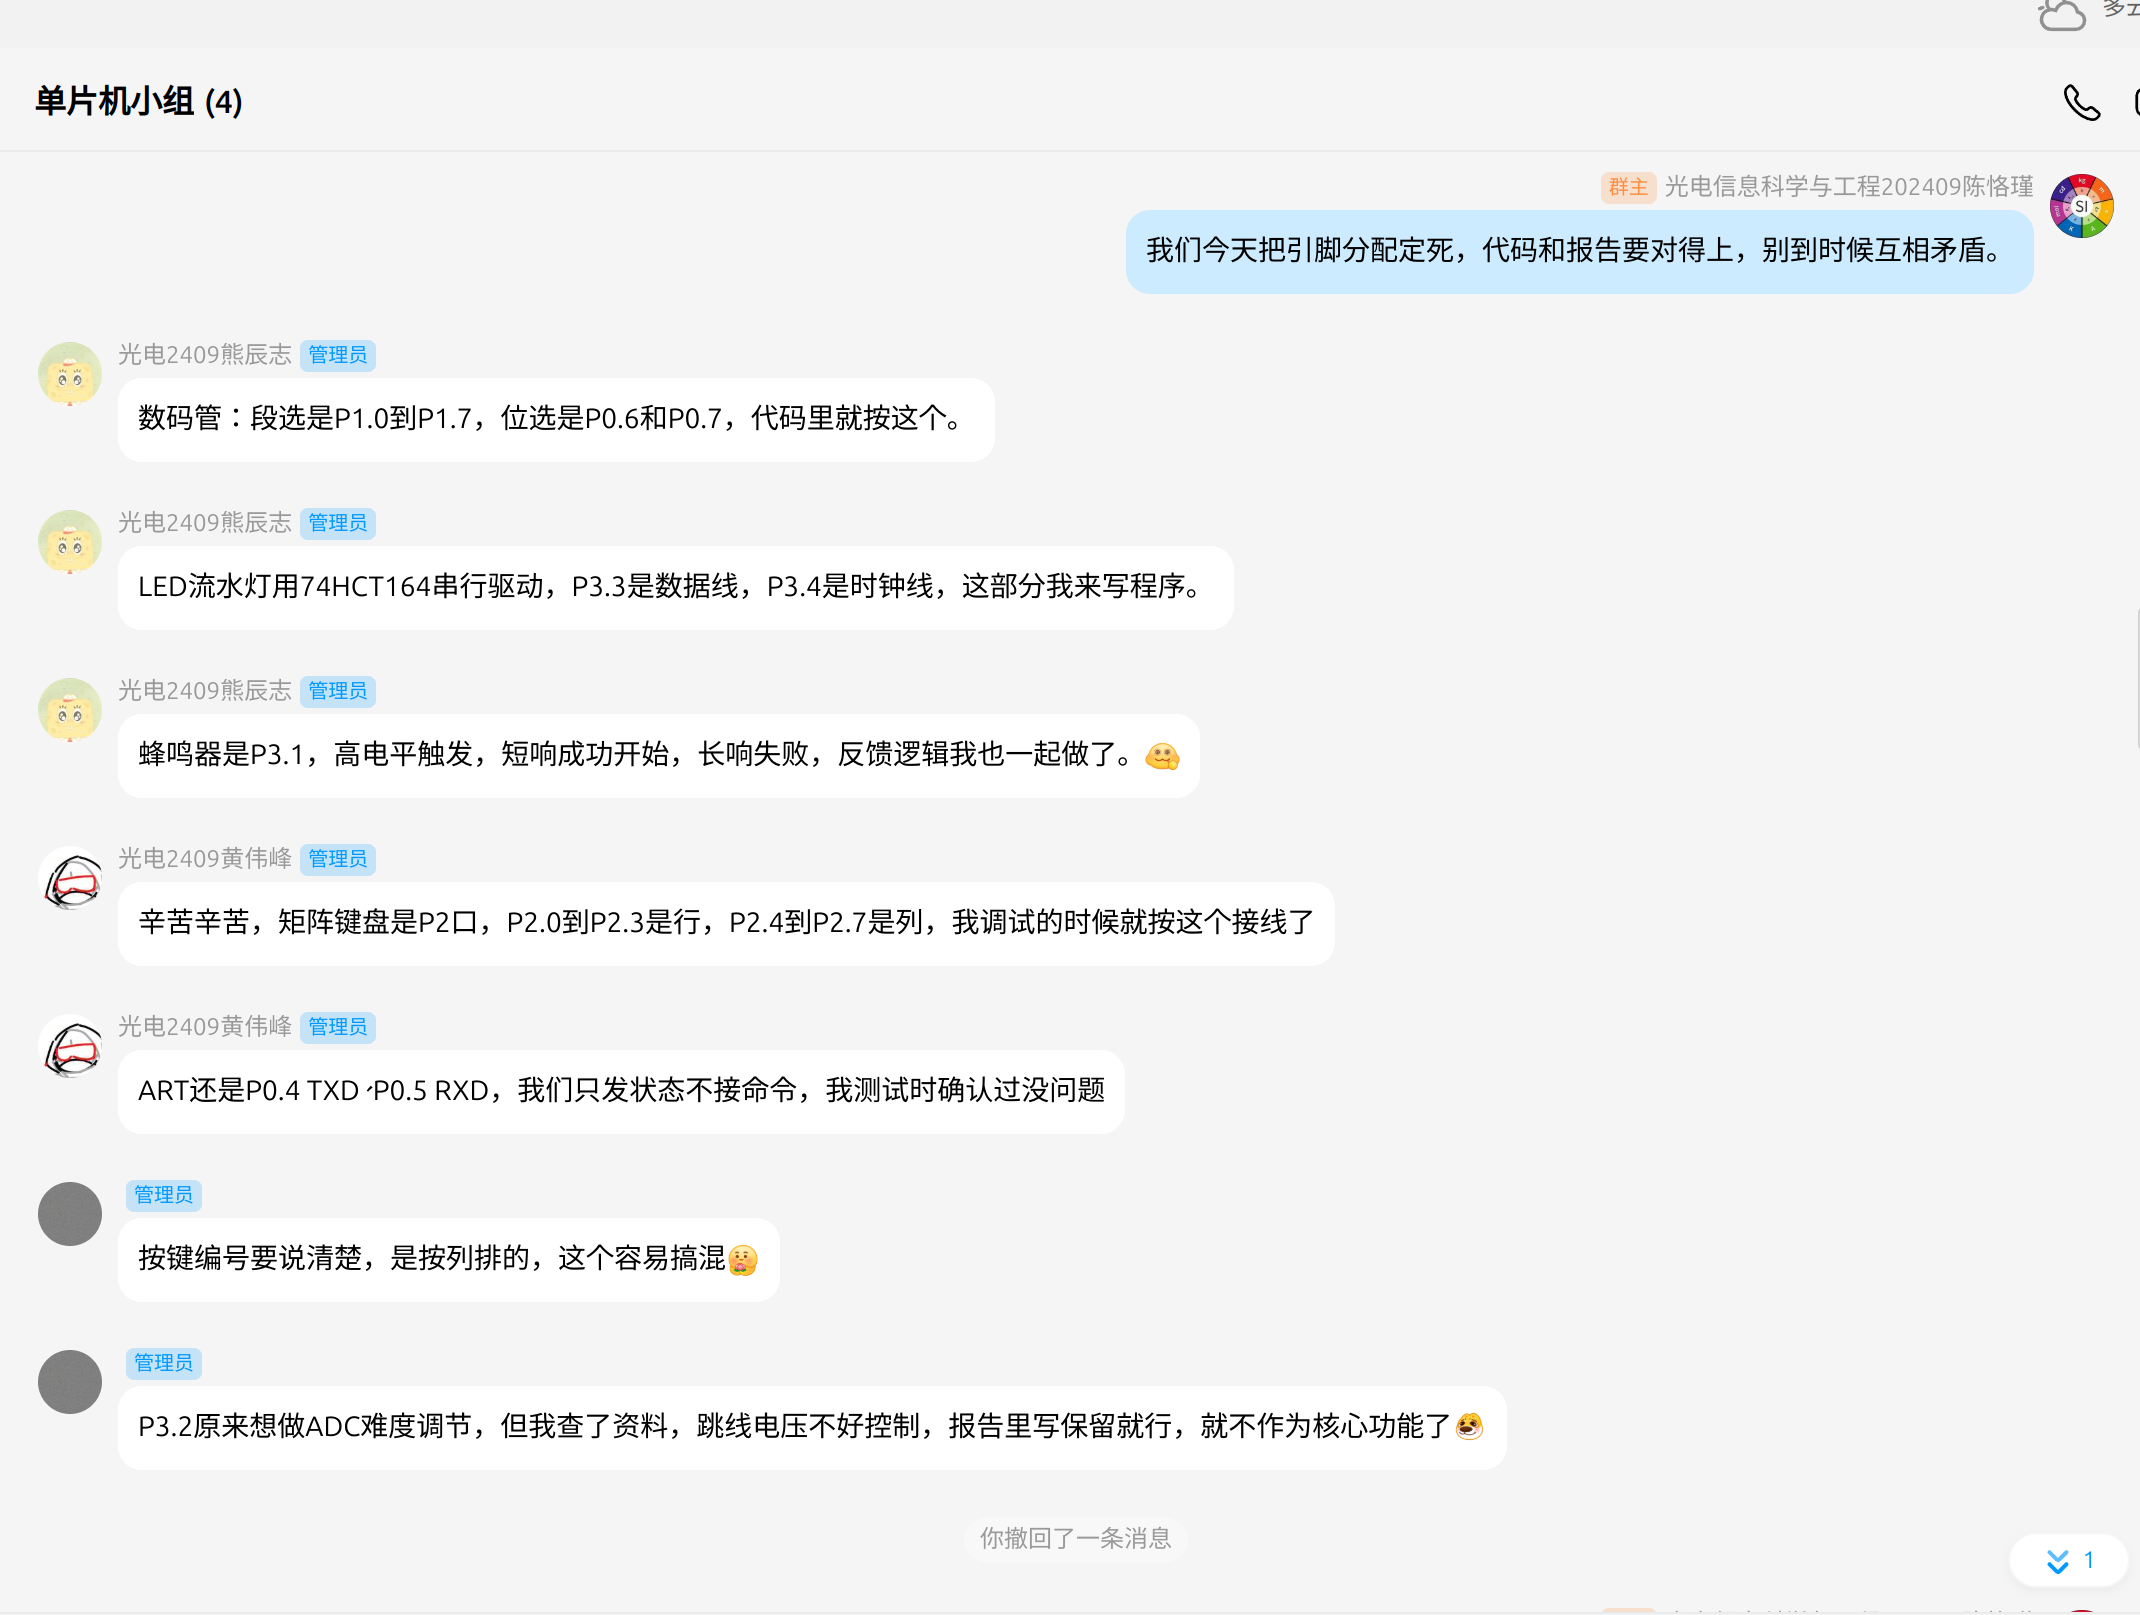
\includegraphics[width=\textwidth,height=0.82\textheight,keepaspectratio]{figures/screenshots/3-1.png}
\captionof{figure}{第三次讨论截图1}
\end{center}

\begin{center}
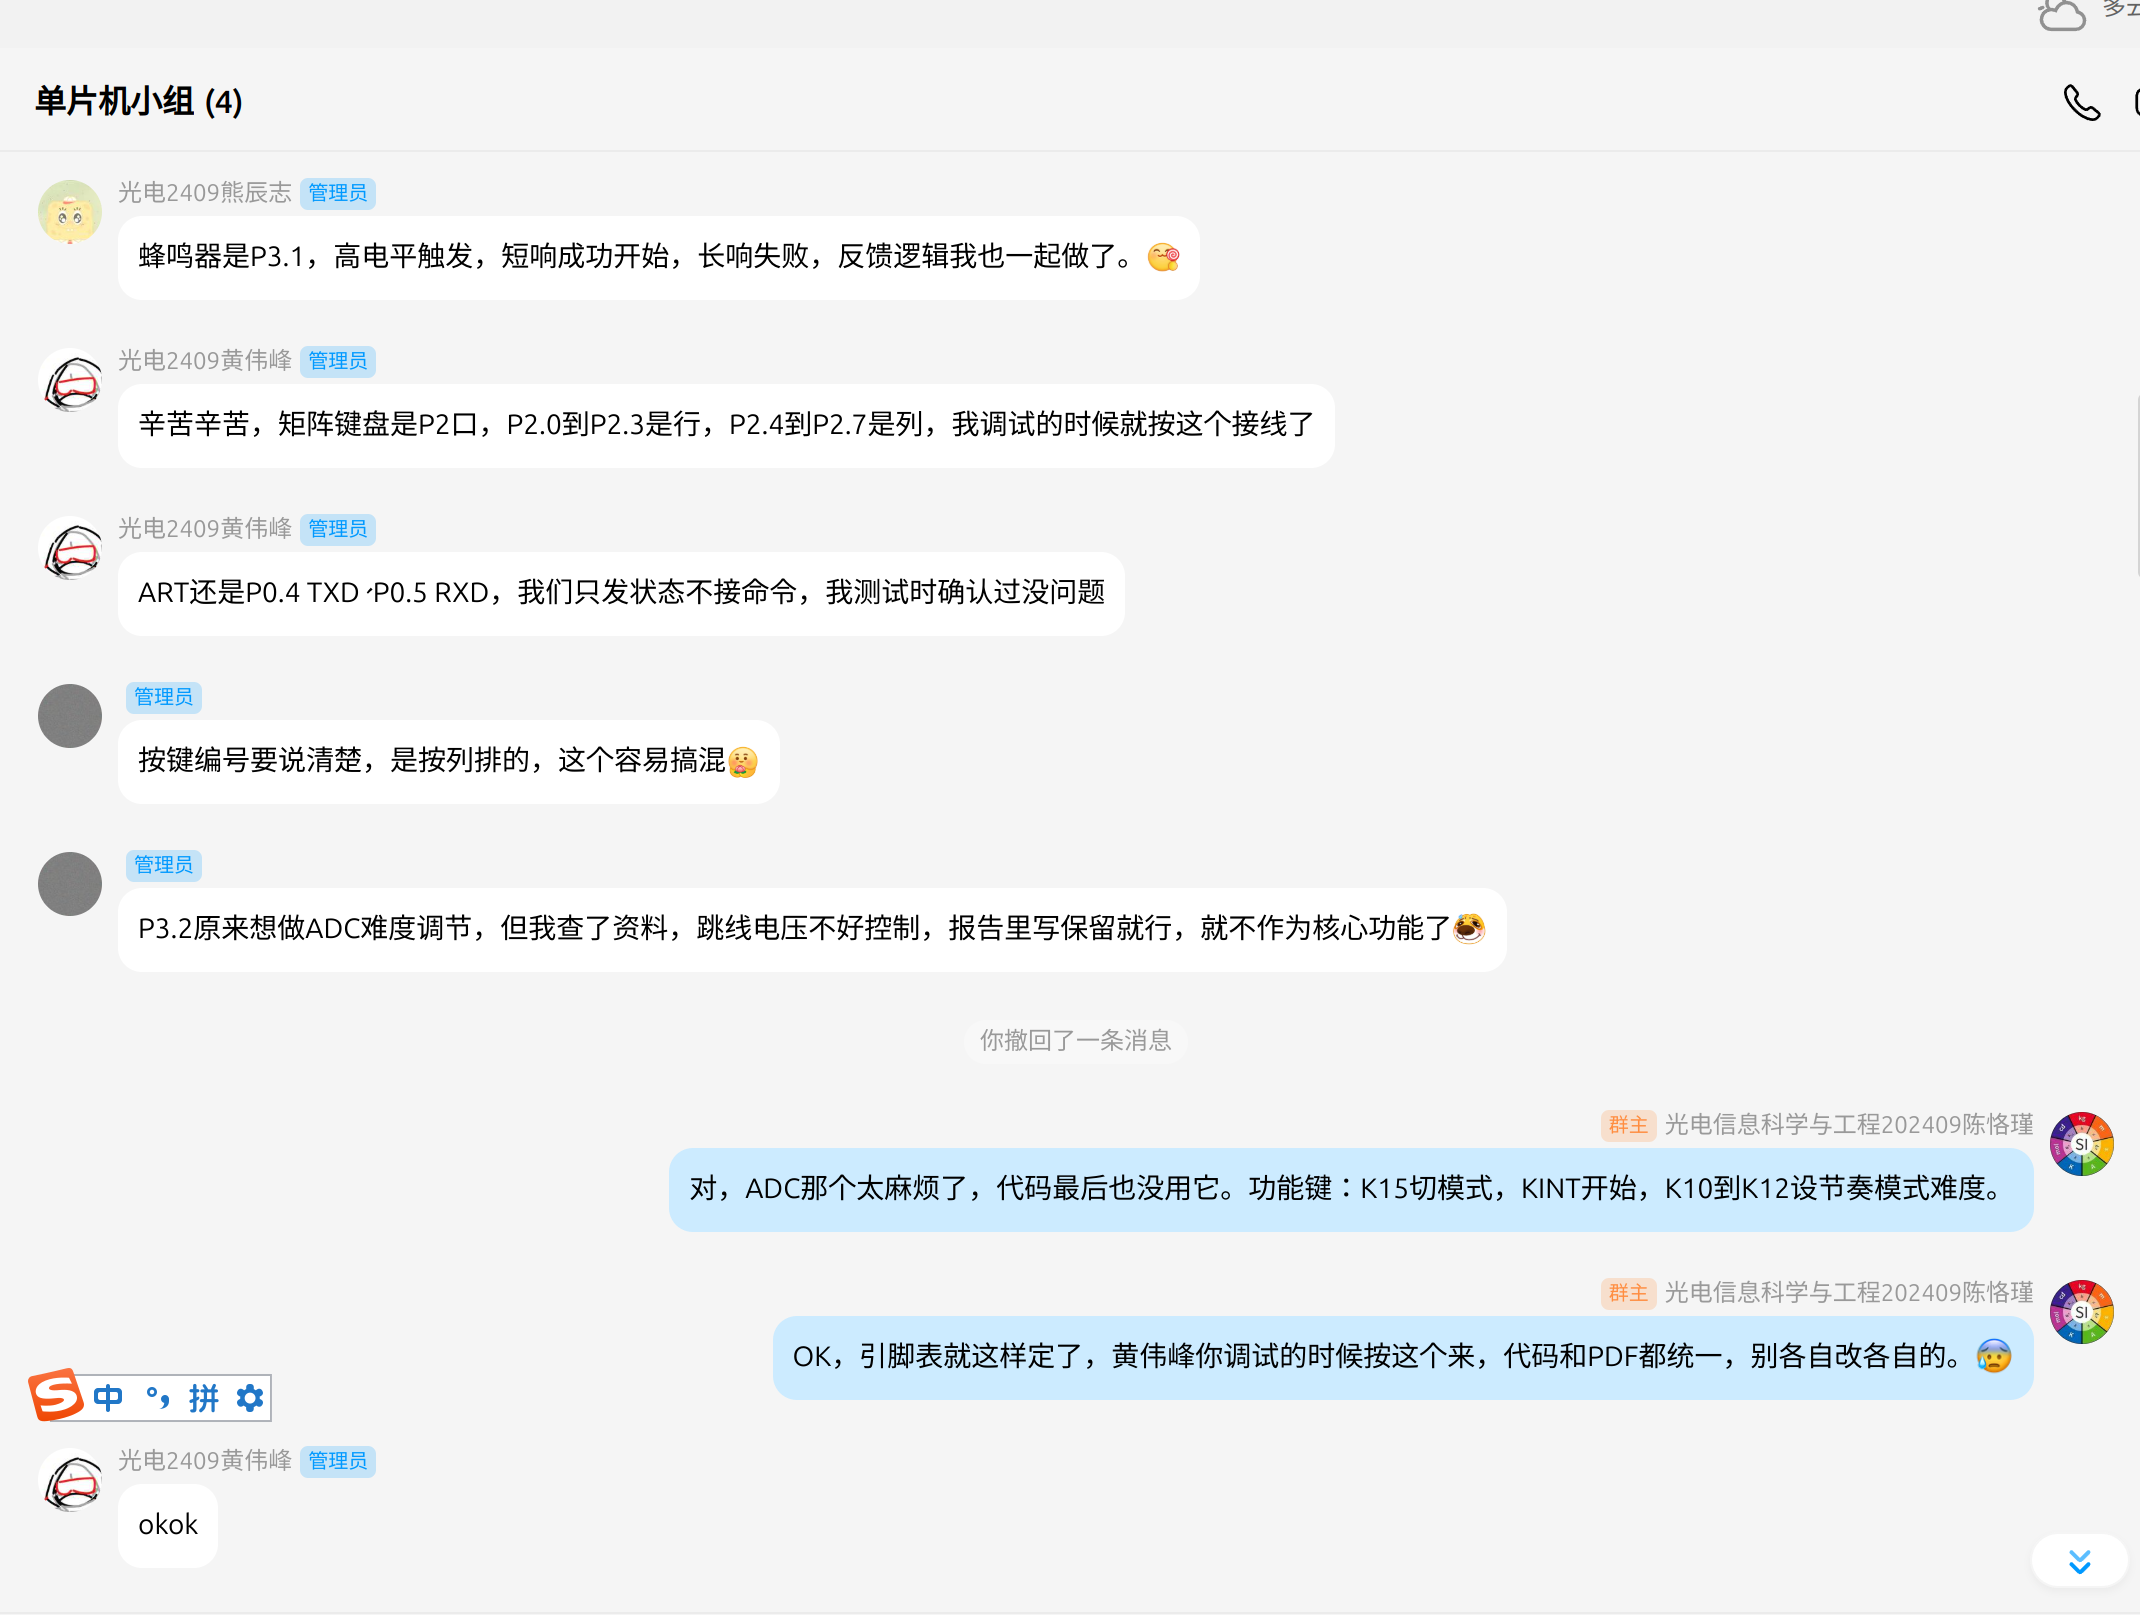
\includegraphics[width=\textwidth,height=0.82\textheight,keepaspectratio]{figures/screenshots/3-2.png}
\captionof{figure}{第三次讨论截图2}
\end{center}

\subsection{第四次讨论：软件状态机设计}
组长建议采用“待机--等待--显示目标--游戏--成功/失败”的状态机组织主流程。组员补充节奏模式需要目标灯、分数和速度档位，最终形成反应模式与节奏模式共用主循环、分别处理状态逻辑的双模式结构。

\begin{center}
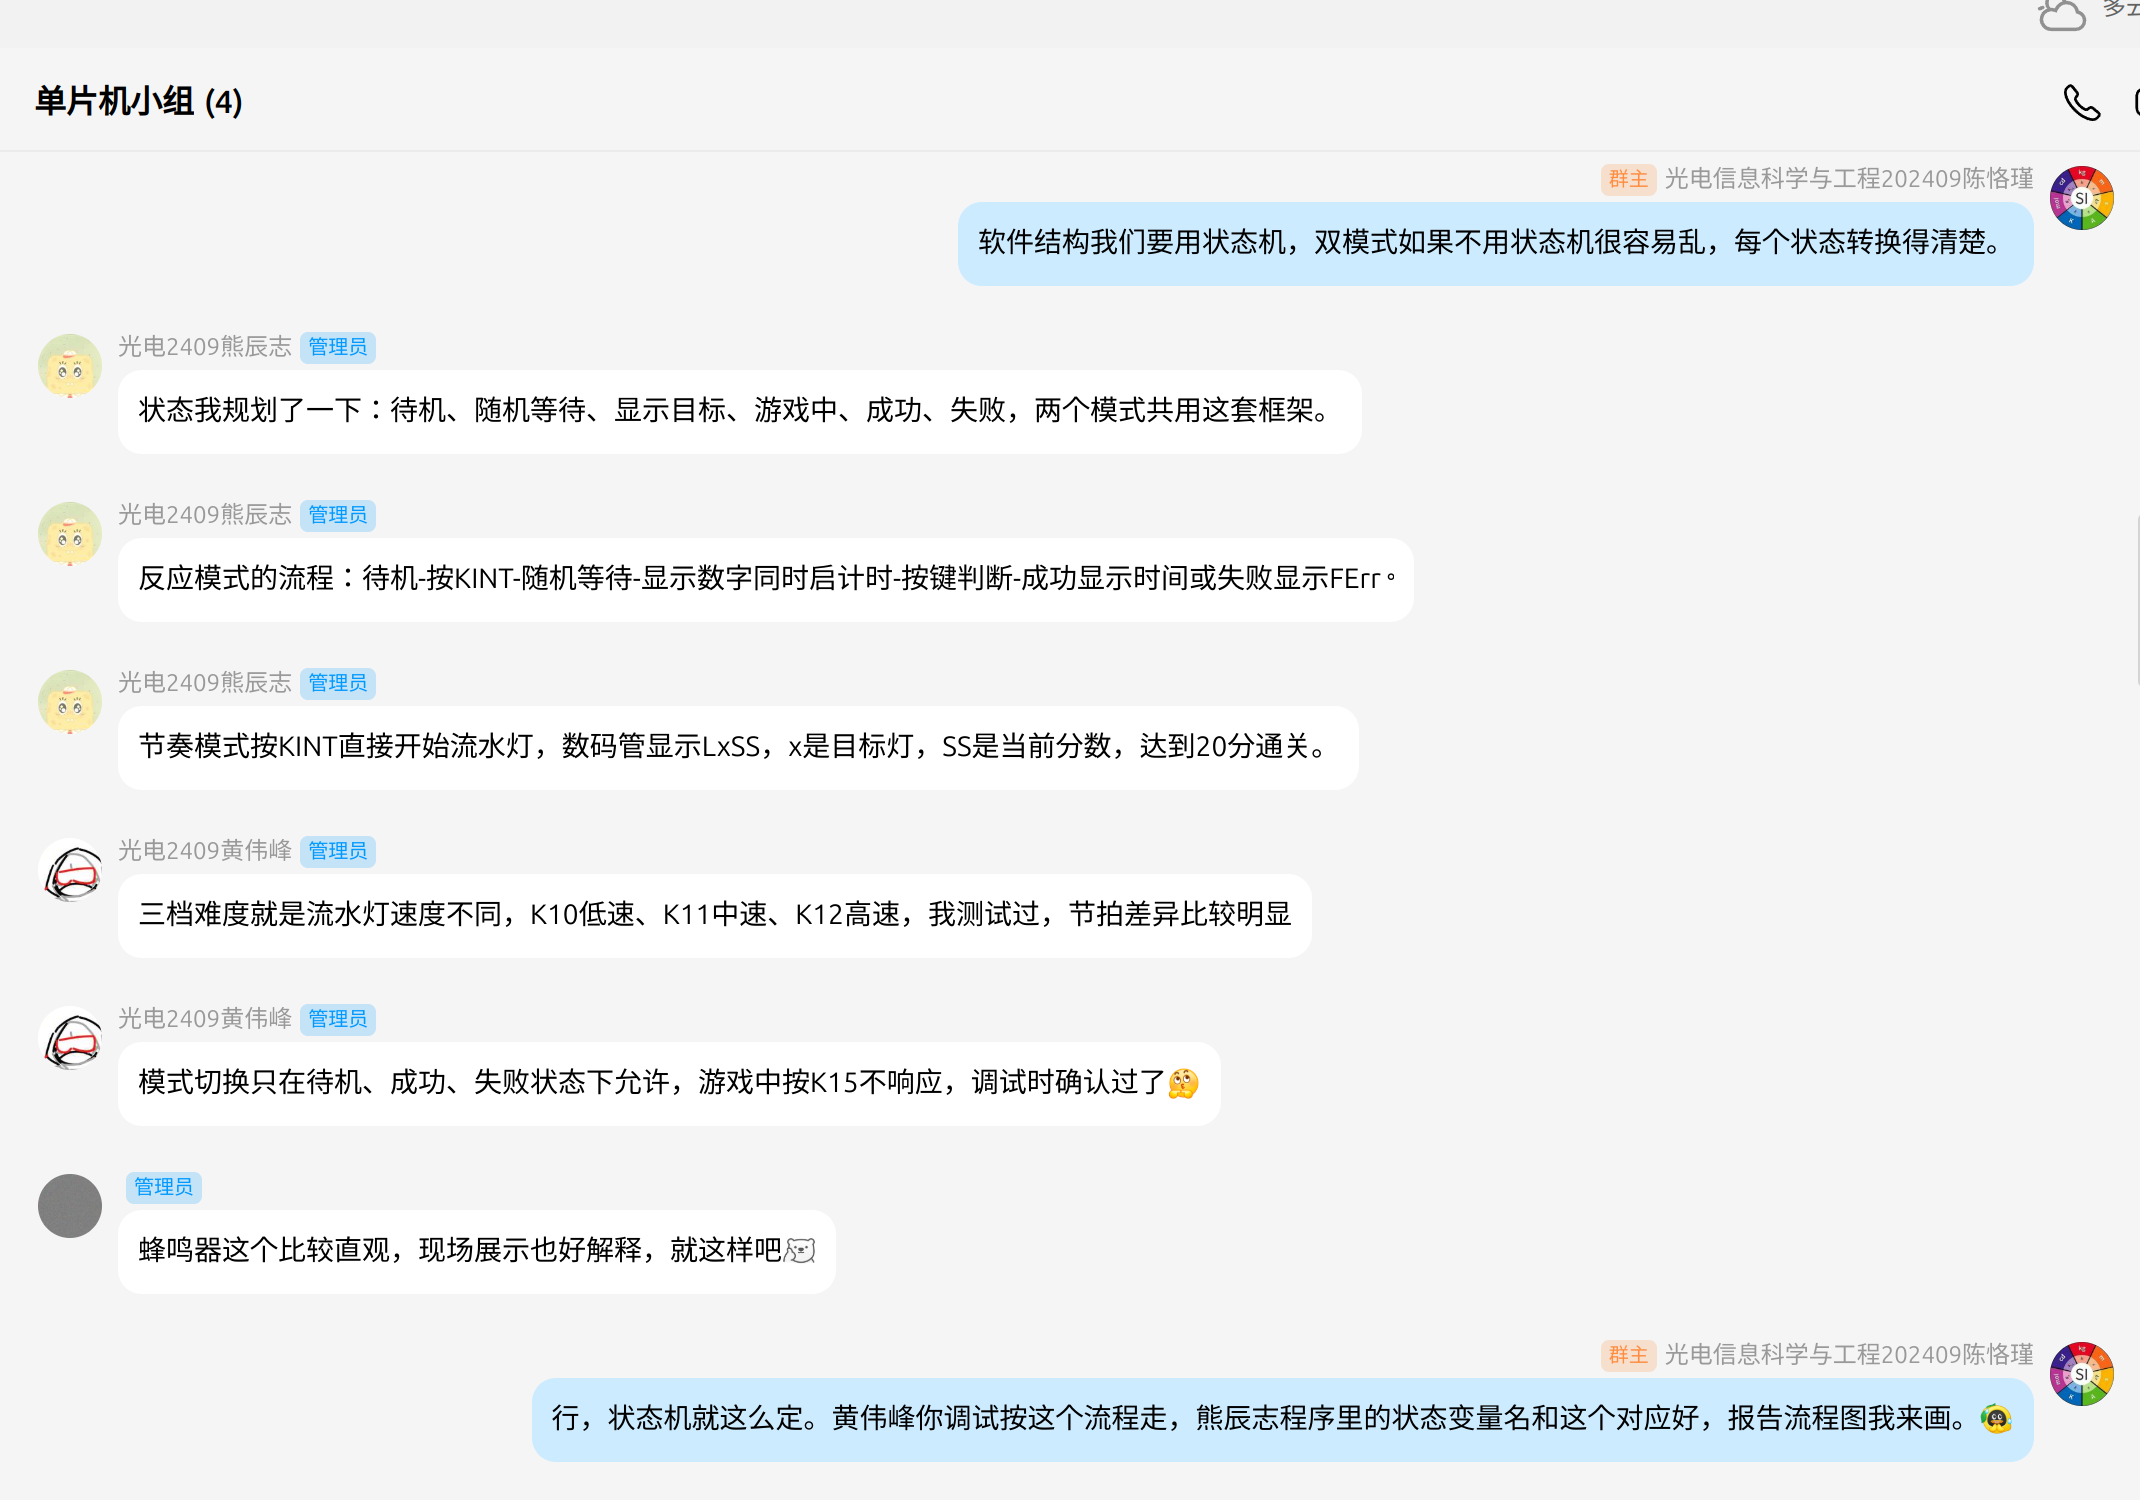
\includegraphics[width=\textwidth,height=0.82\textheight,keepaspectratio]{figures/screenshots/4-1.png}
\captionof{figure}{第四次讨论截图}
\end{center}

\subsection{第五次讨论：核心算法和交互优化}
本次讨论重点是随机等待、反应时间锁存、矩阵键盘消抖和LED软件PWM。小组决定在第一次扫描到按键时锁存反应时间，再进行消抖确认，减少因消抖延时导致的成绩误差；同时加入K10--K12三档节奏难度和K15模式切换。

\begin{center}
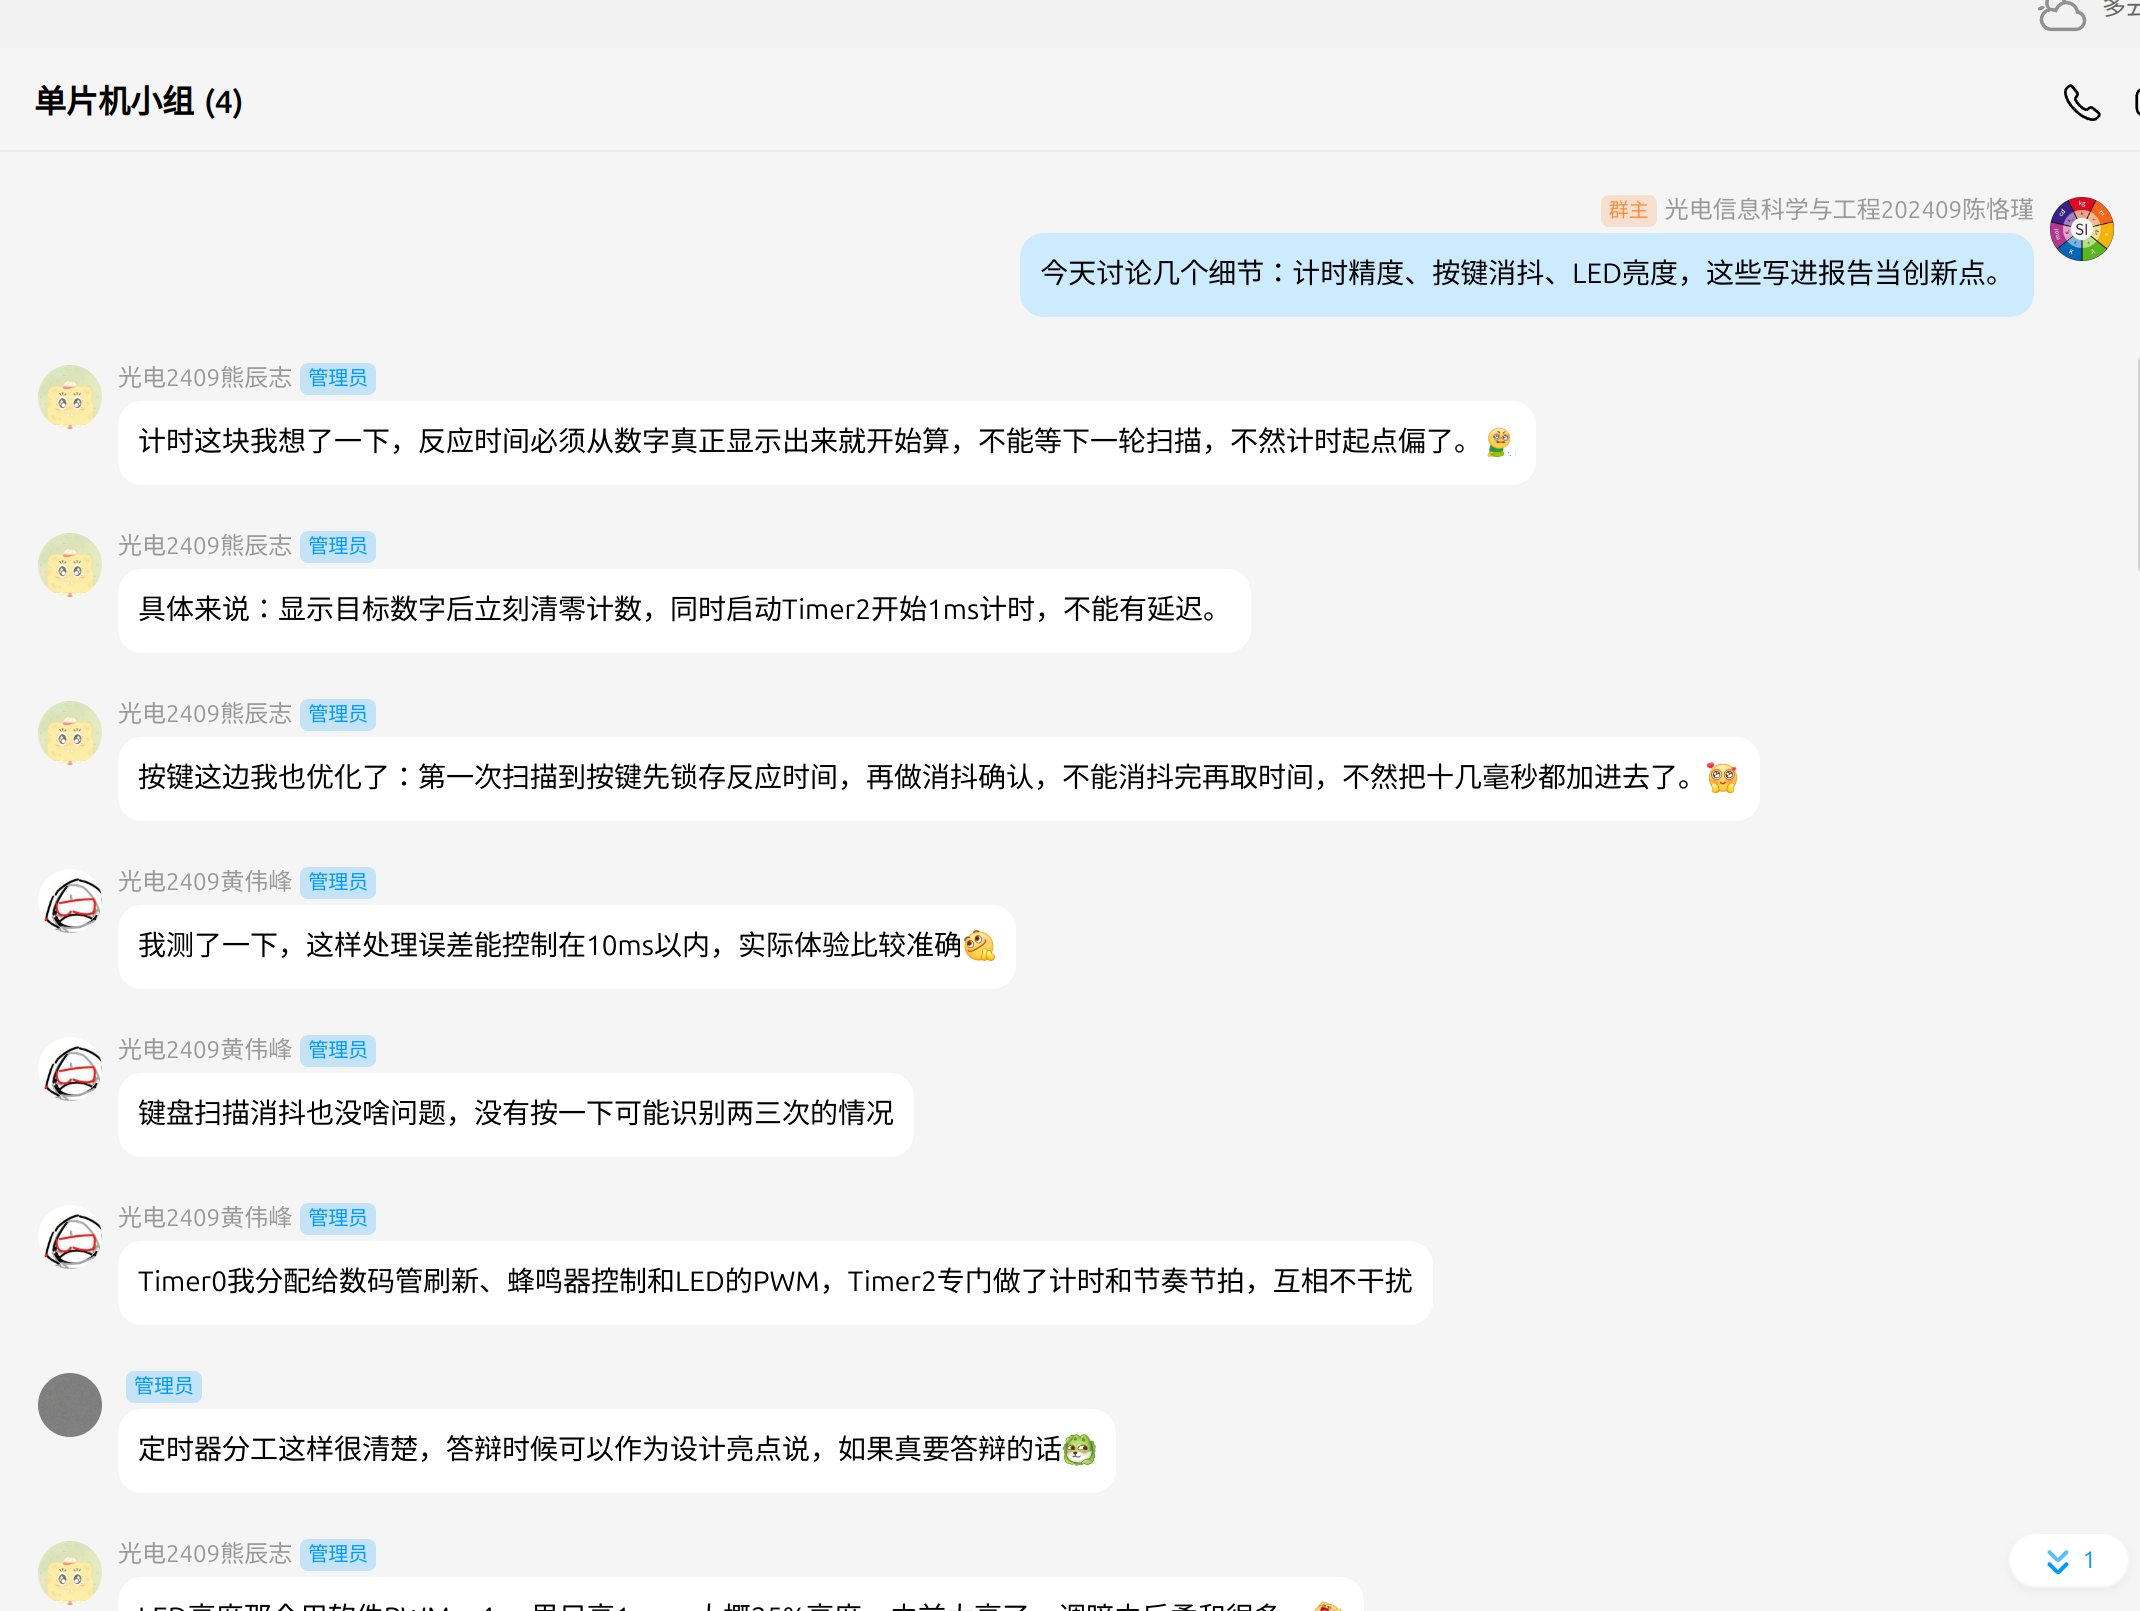
\includegraphics[width=\textwidth,height=0.82\textheight,keepaspectratio]{figures/screenshots/5-1.png}
\captionof{figure}{第五次讨论截图1}
\end{center}

\begin{center}
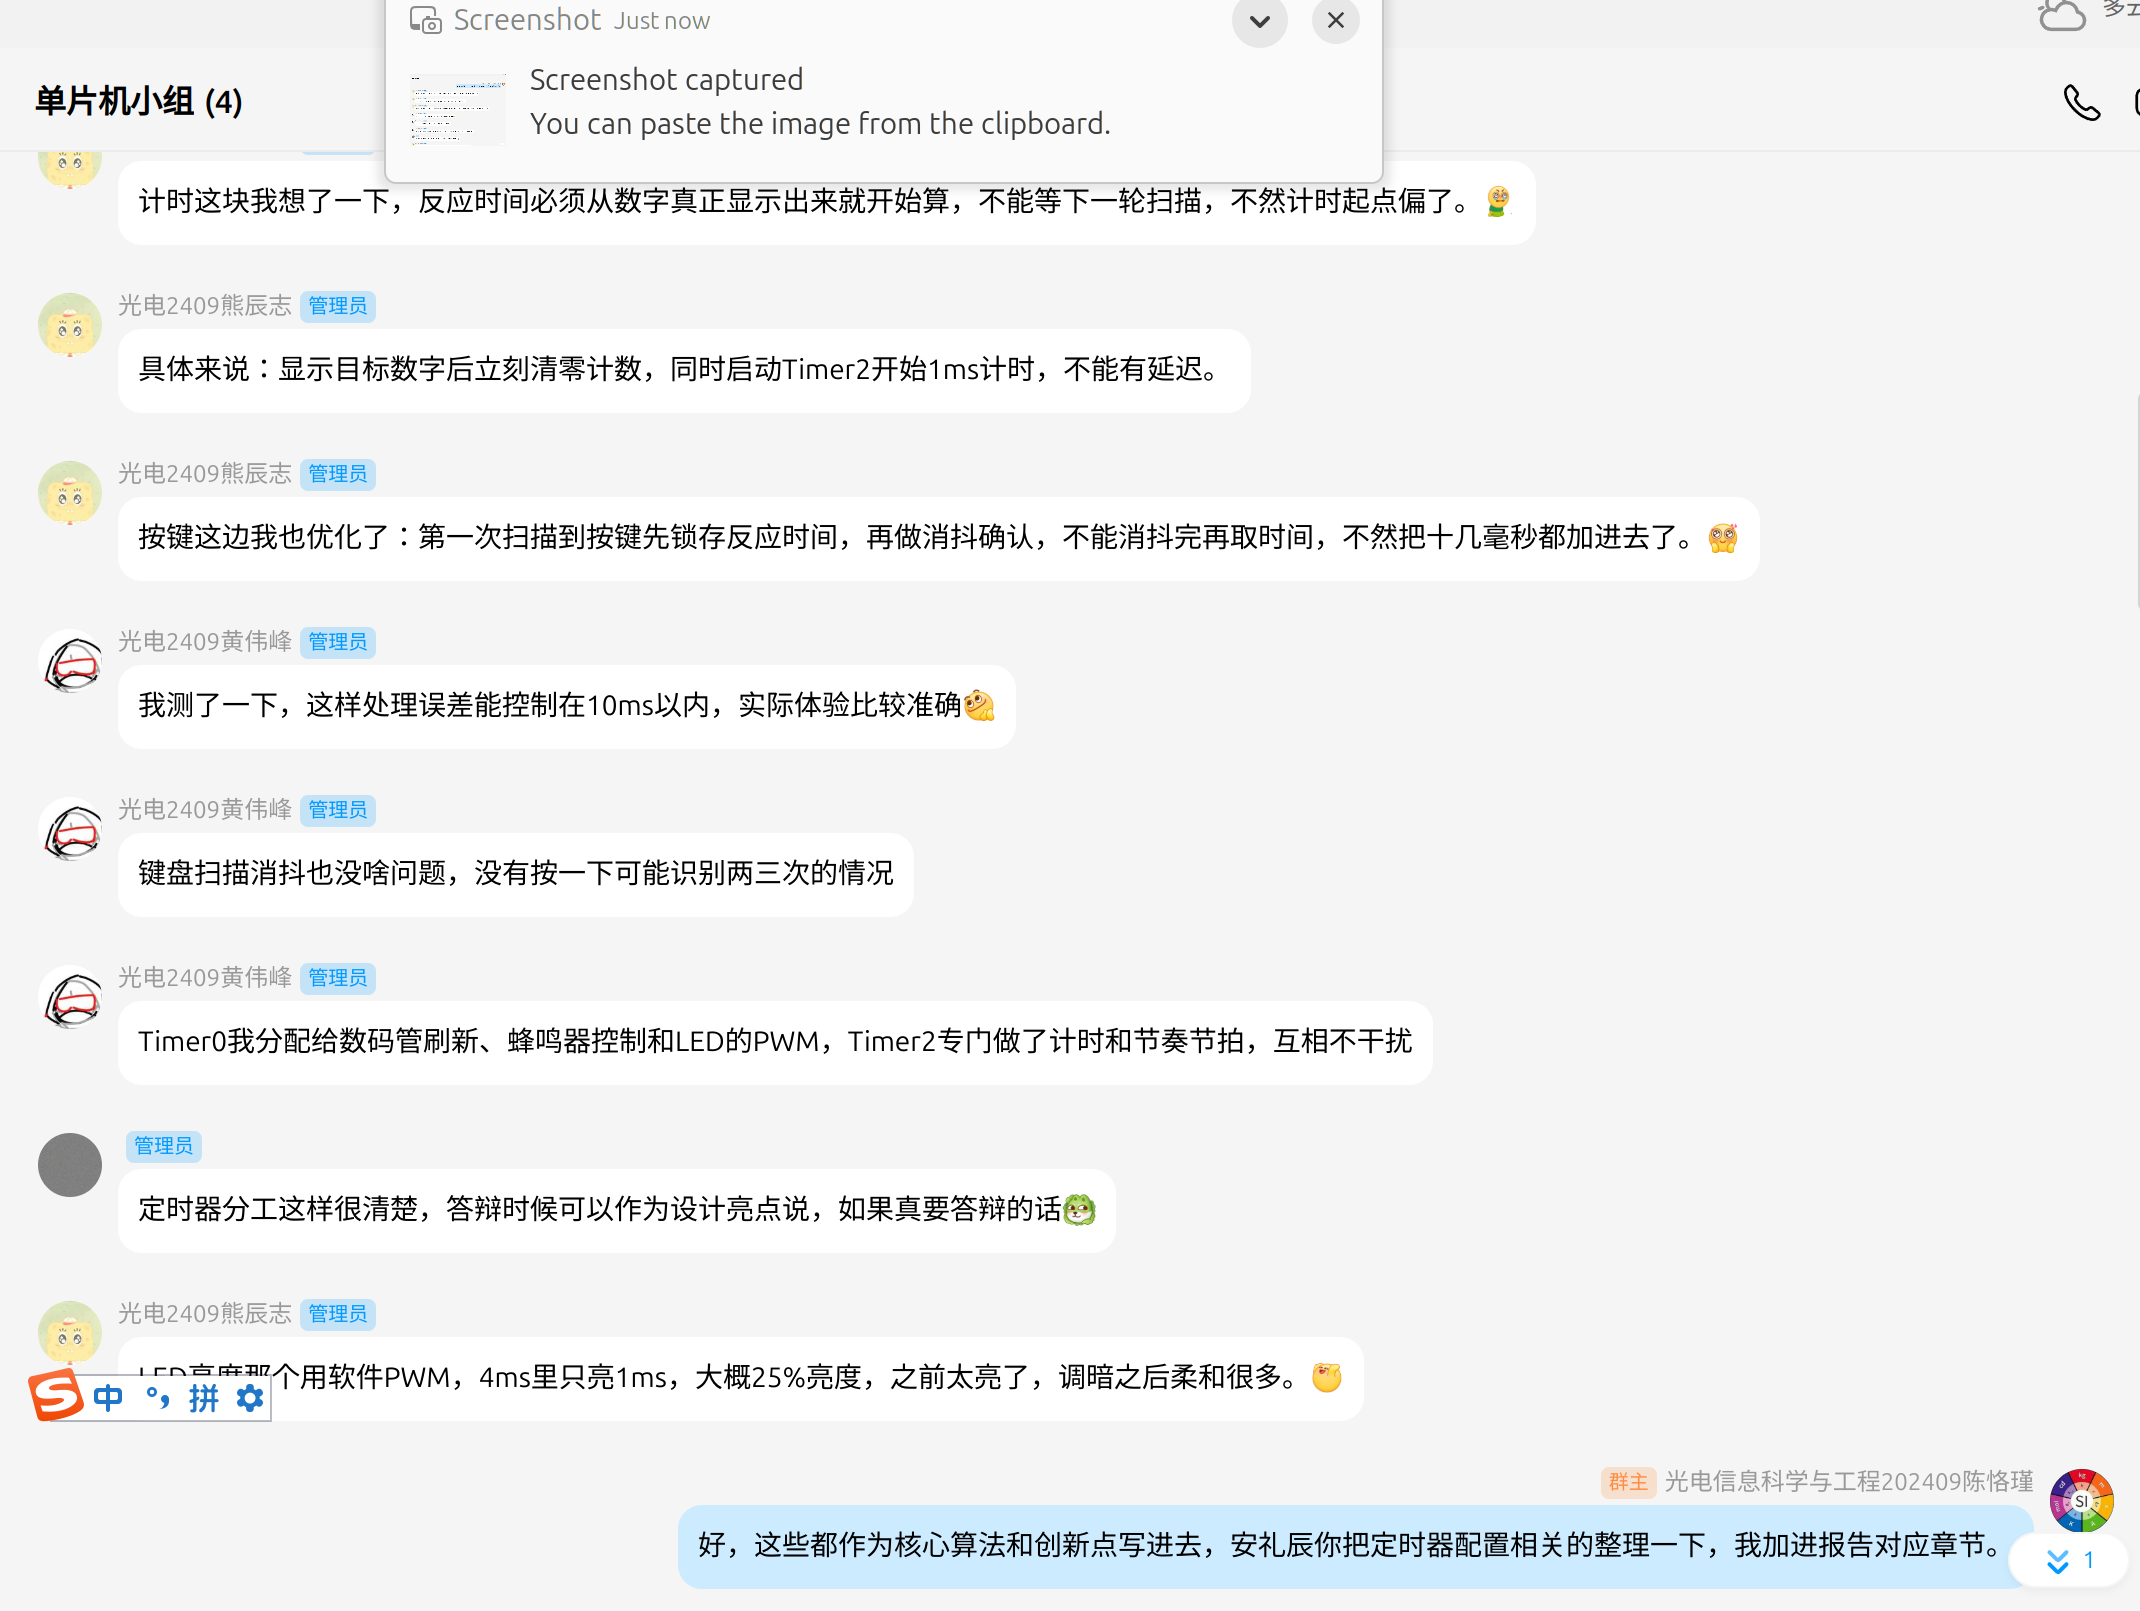
\includegraphics[width=\textwidth,height=0.82\textheight,keepaspectratio]{figures/screenshots/5-2.png}
\captionof{figure}{第五次讨论截图2}
\end{center}

\subsection{第六次讨论：报告和代码整理}
小组对照任务书评分点，补充三个创新点、两类以上人机交互方式、分工贡献说明和附录完整代码清单。代码采用多个ASM模块组织，报告中使用Mermaid流程图说明系统主流程、终端交互流程和中断时基流程。

\begin{center}
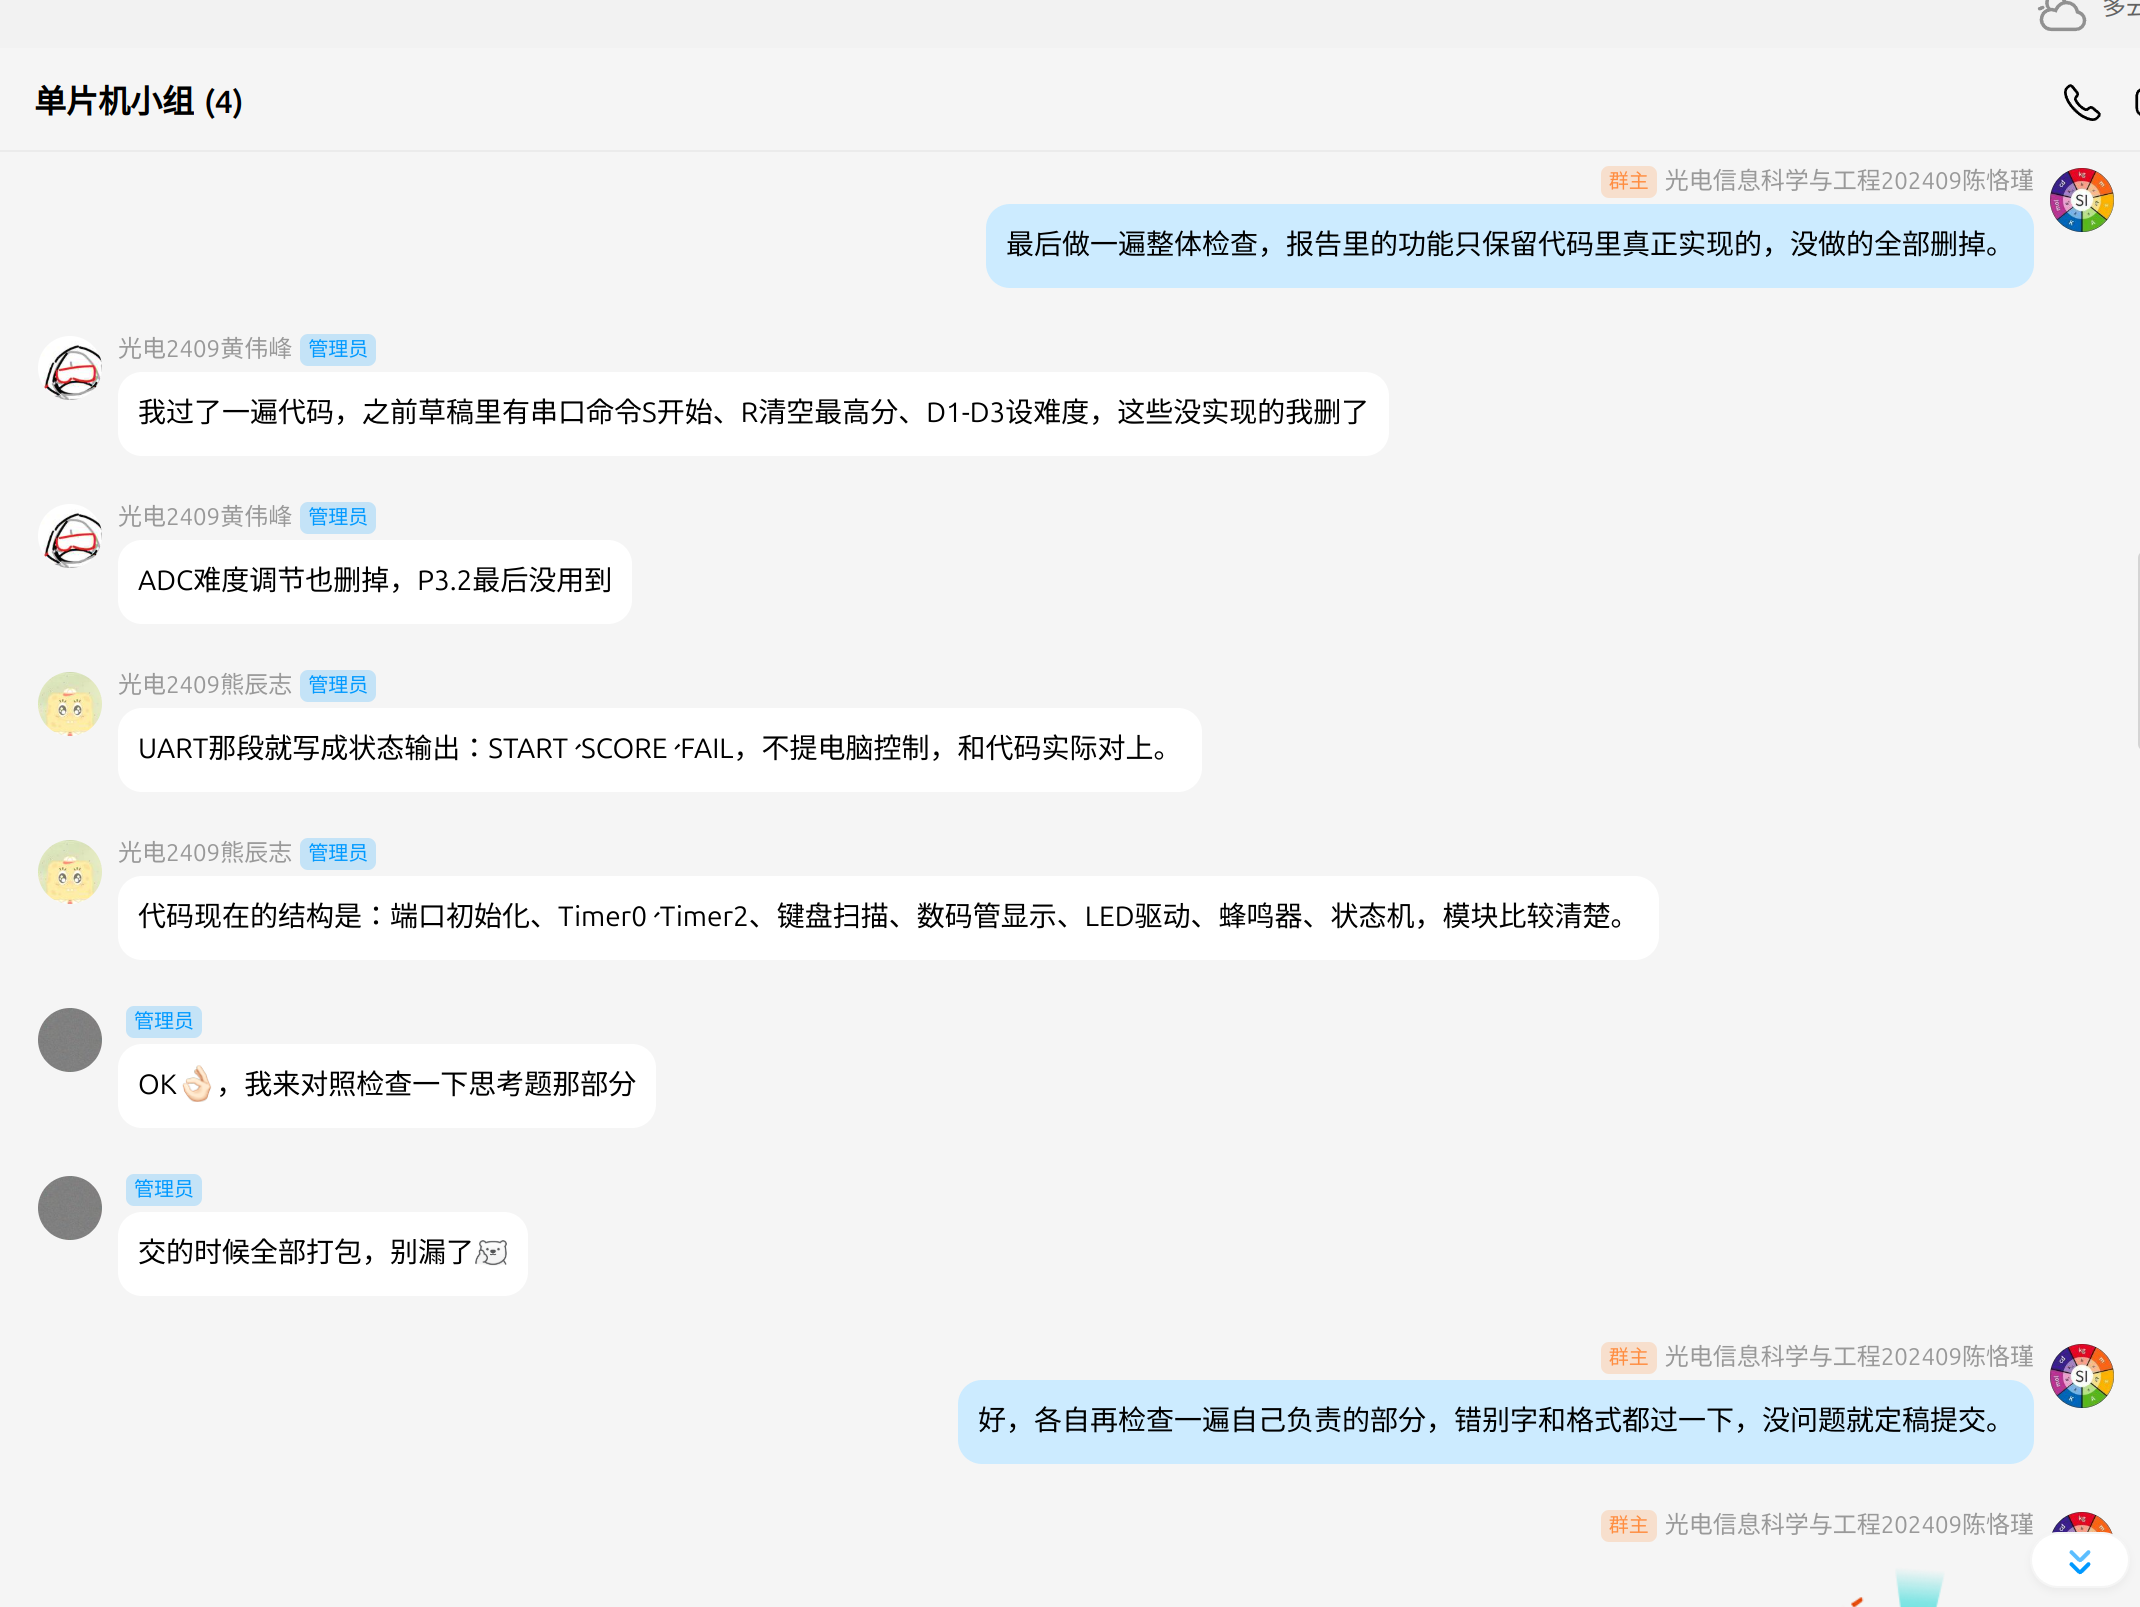
\includegraphics[width=\textwidth,height=0.82\textheight,keepaspectratio]{figures/screenshots/6-1.png}
\captionof{figure}{第六次讨论截图}
\end{center}

\section{项目总结和个人贡献表述}

\subsection{项目预期成果和总结感悟}
本项目预期完成一个基于C8051F310开发板的可运行原型机。上电后系统进入待机状态；用户可通过K15选择反应力测试或节奏挑战，通过K10--K12设置节奏难度；按下KINT后开始游戏；玩家根据数码管和LED提示按键；系统测量反应时间或统计节奏得分，并给出声光反馈；UART向电脑输出START、SCORE和FAIL等状态信息。该作品把多个基础实验整合成一个完整互动系统，既有娱乐性，也能体现单片机综合设计能力。

通过本项目，小组成员能够进一步理解C8051F310作为SoC型单片机的特点，掌握定时器中断、矩阵键盘扫描、动态数码管显示、串口通信、LED串行驱动和软件PWM调光的综合应用。项目也训练了团队分工、方案讨论、问题定位和现场演示表达能力。

\subsection{组长及组员分工和贡献描述}
组长 陈恪瑾：贡献比例30\%。负责确定项目主题，组织讨论，完成系统总体框图、软件流程、报告统稿和现场展示说明，并全程参与其他任务。\par
组员 熊辰志：贡献比例24\%。主要负责设计键盘扫描、数码管显示、LED流水灯、蜂鸣器提示和反应时间测量程序。\par
组员 黄伟峰：贡献比例23\%。主要负责整理ASM代码并调试硬件设备，记录相关的测试数据并反馈，配合修改程序。\par
组员 安礼辰：贡献比例23\%。主要负责查阅 C8051F310 资料，完成思考题解答，整理IO配置、UART 连接和定时器时钟相关内容。\par

\appendix
\section{UART串口连接说明}
开发板UART接口位于J3，接口电平为3.3V TTL。连接USB-TTL模块时，开发板TXD接USB-TTL的RXD，开发板RXD接USB-TTL的TXD，GND必须共地。具体如下：

\begin{center}
\begin{tabular}{lll}
\toprule
开发板信号 & 引脚/接口 & USB-TTL模块连接 \\
\midrule
TXD & P0.4 / J3-1 & RXD \\
GND & J3-2 & GND \\
RXD & P0.5 / J3-3 & TXD \\
\bottomrule
\end{tabular}
\end{center}

推荐串口参数为9600 bps、8位数据位、无校验、1位停止位，即9600, 8N1。程序使用Timer1方式2作为UART0波特率发生器，在24.5MHz系统时钟下令Timer1使用SYSCLK并设置TH1=0xB0，可得到约9570bps，接近9600bps，实际串口助手按9600bps设置即可。

\clearpage
\section{完整ASM代码清单}
\label{app:code}
本附录收录本项目使用的完整汇编代码和头文件。

\subsection{芯片寄存器头文件}
\lstinputlisting[style=asmstyle,caption={C8051F310.INC}]{codes/Core/Inc/C8051F310.INC}

\subsection{项目公共定义}
\lstinputlisting[style=asmstyle,caption={reaction\_game.inc}]{codes/Core/Inc/reaction_game.inc}

\subsection{顶层入口与中断向量}
\lstinputlisting[style=asmstyle,caption={reaction\_game.asm}]{codes/Core/Src/reaction_game.asm}
\lstinputlisting[style=asmstyle,caption={vectors.asm}]{codes/Core/Src/vectors.asm}

\subsection{初始化与主循环}
\lstinputlisting[style=asmstyle,caption={init.asm}]{codes/Core/Src/init.asm}
\lstinputlisting[style=asmstyle,caption={main.asm}]{codes/Core/Src/main.asm}

\subsection{游戏状态机与中断服务}
\lstinputlisting[style=asmstyle,caption={game\_logic.asm}]{codes/Core/Src/game_logic.asm}
\lstinputlisting[style=asmstyle,caption={isr.asm}]{codes/Core/Src/isr.asm}

\subsection{显示、键盘、LED和UART模块}
\lstinputlisting[style=asmstyle,caption={display.asm}]{codes/Core/Src/display.asm}
\lstinputlisting[style=asmstyle,caption={keypad.asm}]{codes/Core/Src/keypad.asm}
\lstinputlisting[style=asmstyle,caption={led\_bar.asm}]{codes/Core/Src/led_bar.asm}
\lstinputlisting[style=asmstyle,caption={uart.asm}]{codes/Core/Src/uart.asm}

\subsection{辅助逻辑与查找表}
\lstinputlisting[style=asmstyle,caption={random\_score.asm}]{codes/Core/Src/random_score.asm}
\lstinputlisting[style=asmstyle,caption={tables.asm}]{codes/Core/Src/tables.asm}

\end{document}
